\section{Desarrollo del sistema.}

En esta sección vamos a dar paso al desarrollo del proyecto, en primer lugar hablaremos sobre la implementación de la red
blockchain en las Raspberry previamente configuradas, para pasar al desarrollo de la API basada en GraphQL con NodeJS y 
posteriormente a la interfaz de usuario con Gatsby y React.  

\subsection{Configuración y creación de la topología de la red.}

Para el montaje de la red Blockchain se ha utilizado 3 RaspberrY Pi 4 Modelo B+ 2GB, que servirán como nodos principales.

\vspace{5mm}

\noindent El sistema operativo utilizado es Ubuntu Server 18.04 \cite{ubuntu-rasp} la versión de 64-bit, que se puede 
encontrar en la página oficial de Raspberry \cite{rasp-official-page}. Para la instalación seguimos los pasos aconsejados 
en la misma página de instalación de Ubuntu. Necesitaremos:

\begin{itemize}
  \item Tarjeta microSD.
  \item Imagen de Ubuntu Server.
\end{itemize}

\noindent Una vez descargada la imagen de Ubuntu Server vamos a crear un punto de arranque en la tarjeta microSD.

\vspace{5mm}

\noindent Desde una terminal ejecutamos los siguientes comandos:

\begin{lstlisting}[language=bash]
  $ diskutil unmountDisk <sdcard>
  $ sudo sh -c 'gunzip -c <imagen> | sudo dd of=<sdcard> bs=32m'
\end{lstlisting}

\vspace{5mm}

\noindent Una vez instalado el sistema operativo, vamos a establecer la dirección estática a cada una de las Raspberry
para evitar la asignación por DHCP, para ello módificamos el fichero \say{/etc/netplan/50-cloud-init.yaml} con la 
siguiente configuración \cite{configure-static-ip}:

\vspace{5mm}

\begin{lstlisting}
  network:
  renderer: networkd
  ethernets:
      eth0:
          addresses: [<direccion>/<mascara>]
          gateway4: <default gateway>
          nameservers:
              addresses: [<direccion_dns>]
  version: 2
\end{lstlisting}

\vspace{10mm}

\noindent Y aplicamos los cambios con el siguiente comando:

\begin{lstlisting}[language=bash]
  $ sudo netplan apply
\end{lstlisting}

\vspace{5mm}

\noindent En la siguiente imagen se muestra la topología final de la red (ver fig.\ref{fig:topologia-red}):

\begin{figure}[ht!]
  \centering
  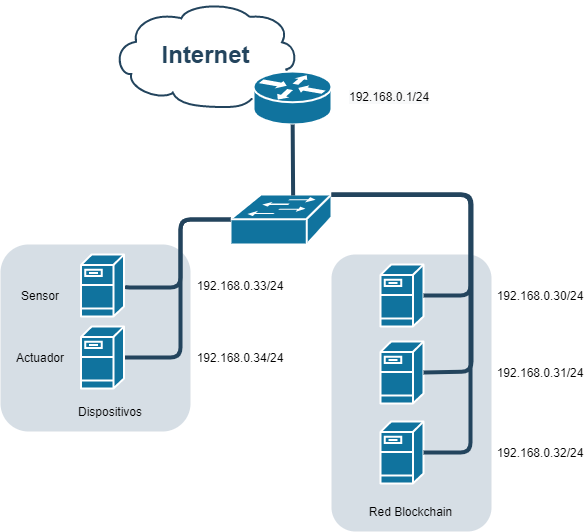
\includegraphics[width=8cm]{imagenes/desarrollo/topologia_red}
  \caption{Topología de la red.}
  \label{fig:topologia-red}
\end{figure}

\begin{figure}[ht!]
  \centering
  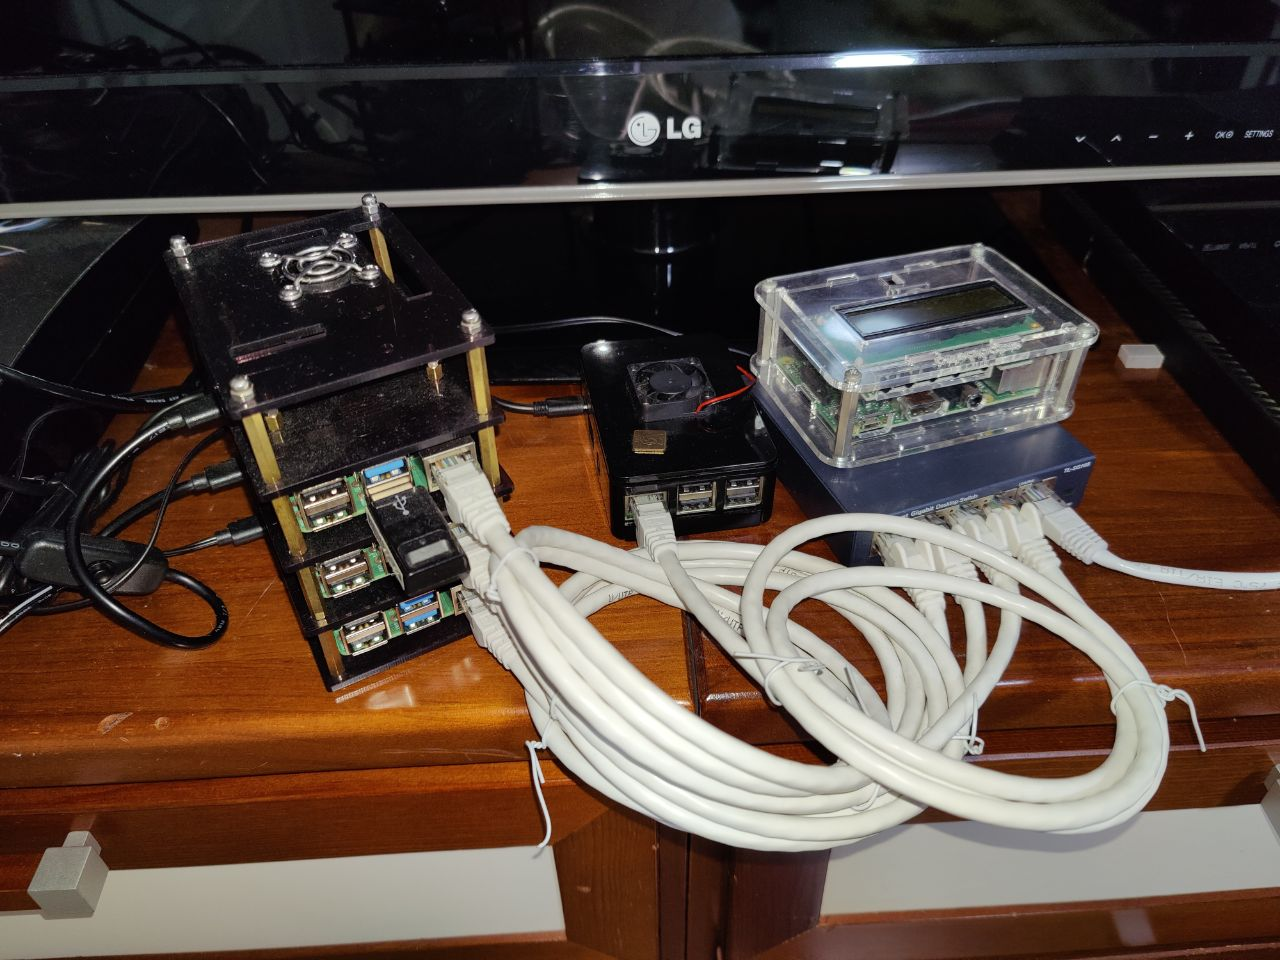
\includegraphics[width=10cm]{imagenes/desarrollo/foto_raspberry}
  \caption{Captura de las Raspberry Pi.}
  \label{fig:captura-raspberry}
\end{figure}

\subsubsection*{Instalación de Hyperledger Fabric 1.4.4.}

Para la instalación de Hyperledger Fabric (1.4.4) necesitaremos que cada nodo tengan los siguientes requisitos instalados 
\cite{hyperledger-fabric-docs}:

\begin{itemize}
  \item cURL.
  \item Docker version 17.06.2-ce o mayor \cite{install-docker-rasp, set-up-docker-rasp}.
  \item git.
  \item Docker Compose 1.14.0 o mayor \cite{install-docker-rasp, set-up-docker-rasp}.
  \item Go version 1.12.x
  \item Node.js
  \item npm version 5.6.0
  \item Python 2.7
\end{itemize}

\vspace{5mm}

\noindent Una vez instalado los requisitos procedemos a la creación de las imagenes de Hyperledger Fabric a partir de 
los binarios. Actualmente no hay soporte para arquitecturas ARM ya que Hyperledger sólamente soporta las siguientes 
arquitecturas \cite{build-docker-images}:

\begin{itemize}
  \item amd64
  \item s390x
  \item ppc64le
\end{itemize}

\noindent Por tanto el principal objetivo y uno de los obstáculos importantes, es conseguir que Hyperledger Fabric 
se ejecutara en Raspberry Pi. Por ello, realice la construcción de mis propias imagenes de Docker que se pueden 
encontrar en mi DockerHub \cite{dockerhub}. Para ello, he tenido que realizar una serie de cambios en el código fuente
de Hyperledger Fabric que se encuentra distribuido en dos repositorios: \textbf{fabric-baseimage}\footnote{Actualmente, 
este proyecto se encuentra deprecated. \label{fnlabel}} y \textbf{fabric} \cite{fabric-baseimage, fabric}. 

\subsubsection*{fabric-baseimage}

Para poder llevar acabo la construcción de las imágenes Docker y los binarios, he forkeado el repositorio de 
Hyperledger/fabric-baseimage \cite{fabric-baseimage} desde la etiqueta v0.4.18 y he realizado los siguientes 
\href{https://github.com/Thejokeri/fabric-baseimage/commit/f3dfc7bcbdbd62c0c391aa3ce7eeb594ed6a3309}{cambios} para 
construir las imágenes con la última versión de arm64v8. Todos estos cambios se pueden encontrar en la rama \say{project} 
del repositorio \cite{fork-fabric-baseimage}.

\begin{lstlisting}[language=bash]
  $ git clone -b project https://github.com/Thejokeri/fabric-baseimage.git 
  \\ clonamos el repositorio fork desde la rama proyect
\end{lstlisting}

\noindent Con la siguiente orden del Makefile:

\begin{lstlisting}[language=bash]
  $ make docker couchdb kafka zookeeper
\end{lstlisting}

\noindent generamos las imágenes necesarias:

\begin{itemize}
  \item fabric-baseos
  \item fabric-baseimage
  \item fabric-couchdb
  \item fabric-kafka
  \item fabric-zookeeper
\end{itemize}

\subsubsection*{fabric}

Desde el repositorio oficial, clonamos desde la rama v1.4.4:

\begin{lstlisting}[language=bash]
  $ git clone -b v1.4.4 https://github.com/hyperledger/fabric.git
\end{lstlisting}

\noindent Y lanzamos la siguiente orden Makefile, para generar las imágenes restantes de Hyperledger:

\begin{lstlisting}[language=bash]
  $ make native license spelling linter docker
\end{lstlisting}

\begin{itemize}
  \item fabric-tools
  \item fabric-buildenv
  \item fabric-ccenv
  \item orderer
  \item peer
\end{itemize}

\newpage

\noindent El resultado final es el siguiente:

\begin{figure}[ht!]
  \centering
  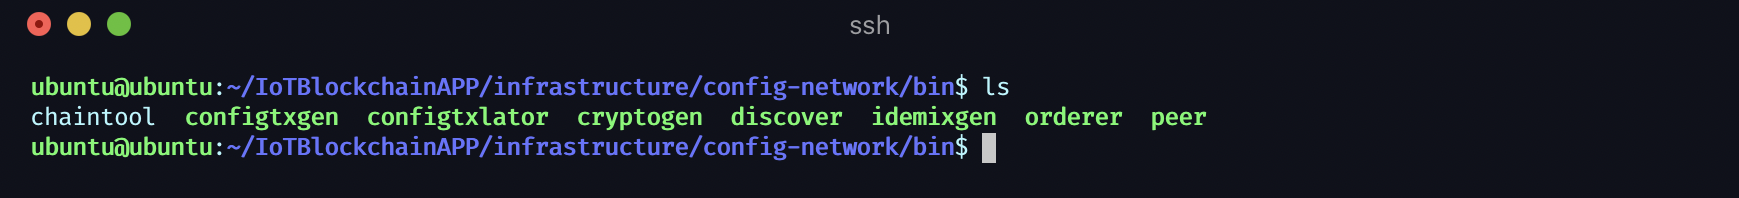
\includegraphics[width=10cm]{imagenes/desarrollo/binarios_fabric}
  \caption{Binarios de Hyperledger Fabric.}
  \label{fig:binarios-fabric}
\end{figure}

\begin{figure}[ht!]
  \centering
  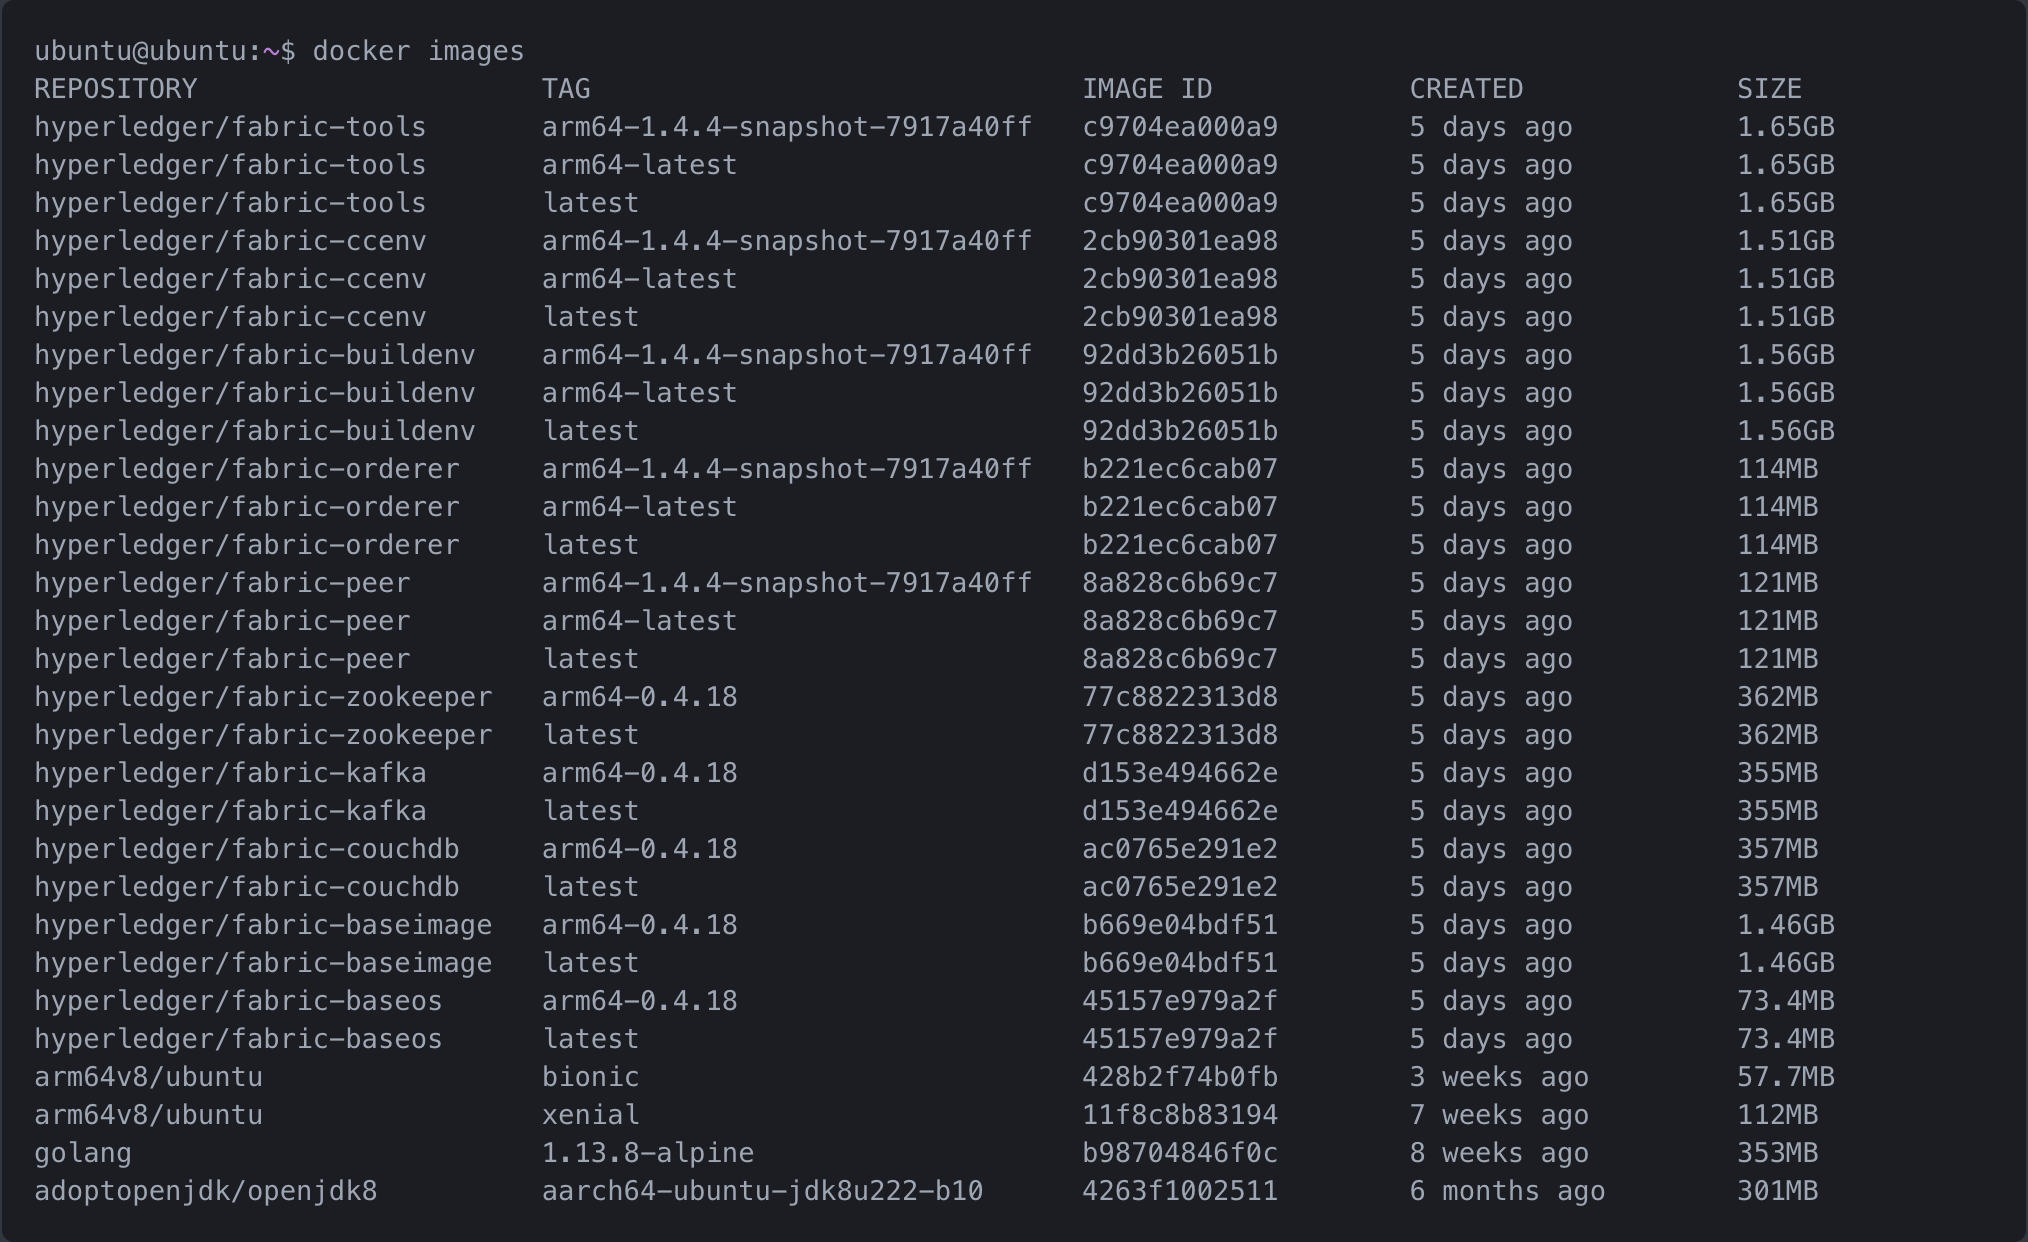
\includegraphics[width=10cm]{imagenes/desarrollo/imagenes_docker}
  \caption{Imagenes Docker de Hyperledger Fabric.}
  \label{fig:imagenes-docker}
\end{figure}

Como se mencionó anteriormente, como vamos a utilizar varias Raspberries como nodos principales de la red Blockchain, 
como un clúster, voy a utilizar Docker Swarm para la orquestación de multiples contenedores dentro de múltiples 
máquinas anfitrionas. Para llevarlo a cabo, nos conectamos al nodo que va a ser el maestro, en este caso va ser 
\textbf{192.168.0.30}, e introducimos el siguiente comando:

\begin{lstlisting}[language=bash]
  $ docker swarm init
\end{lstlisting}

\noindent Este comando genera dos token al azar, una de trabajador y otra de gerente. Cuando unes un nuevo nodo al 
swarm, el nodo se une como un nodo trabajador o gerente basado en el token que usas para unirte al enjambre.

\vspace{5mm}

\noindent Unimos los nodos \textbf{192.168.0.31} y \textbf{192.168.0.32} al swarm con el comando que se genera: 

\begin{lstlisting}[language=bash]
  $ docker swarm join --token SWMTKN-1-XXXX 192.168.0.30:2377
\end{lstlisting}

\newpage

\noindent En la siguiente figura podemos ver los nodos unidos y activos (ver fig. \ref{fig:node-ls-worker}):

\begin{figure}[ht!]
  \centering
  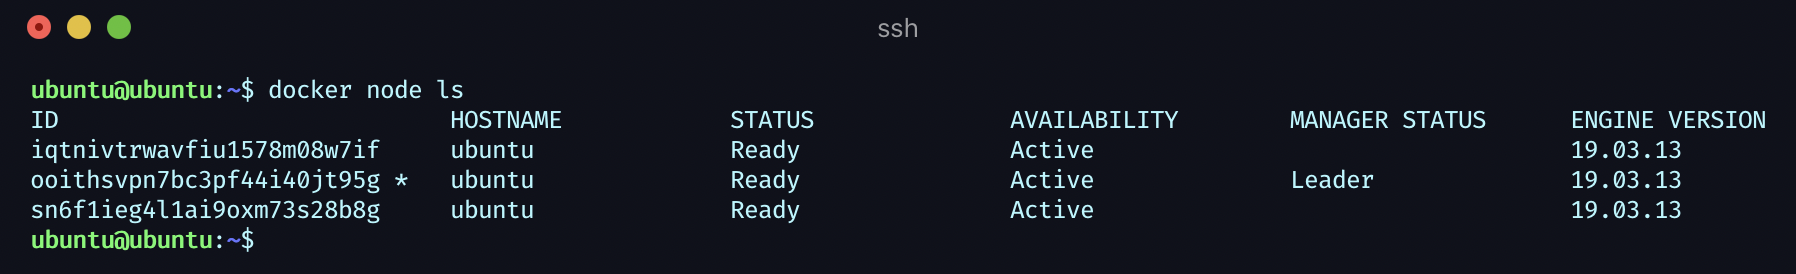
\includegraphics[width=10cm]{imagenes/desarrollo/comandos/node_ls_worker}
  \caption{Nodos de Docker Swarm.}
  \label{fig:node-ls-worker}
\end{figure}

\noindent Con Docker Swarm conseguimos que los contenedores que vayamos a crear para la red Blockchain, se lance de forma 
arbitraria en cada uno de los nodos y no nos tenemos que preocupar en ir levantando cada contenedor uno por uno
en las máquinas. Solamente basta con lanzarlo en el nodo maestro y él se encargará de asignarle los contenedores
a los nodos trabajadores activos, todo en una red privada \cite{hyperledger-fabric-rasp-swarm}.

\vspace{5mm}

Para facilitar el proceso de instalación de prerrequisitos, creación de binarios, imagenes, Docker Swarm, etc. Se ha
creado un script \textbf{setup\_base.sh} que tiene las siguientes opciones:

\begin{lstlisting}[language=bash]
./setup_base.sh \-h
Uso: setup_base.sh [opciones]

opciones:
-h : muestra esta ayuda
-p : instalar prerrequisitos
-f : instalar binarios e imagenes de Hyperlegder Fabric
-s : iniciar Docker Swarm cluster
-d : pull imagenes Docker
-w : muestra las versiones de los prerrequisitos

e.g. setup_base.sh -f
creara los binarios e imagenes de Hyperledger Fabric
\end{lstlisting}

\newpage

\subsection{Implementación de la red Blockchain.}

Después de configurar las Raspberry Pi e instalar los requisitos, vamos a implementar la red Blockchain.
Dentro del repositorio, la estructura de ficheros que rige la infraestructura de la red es la siguiente:

\begin{figure}[ht!]
  \centering
  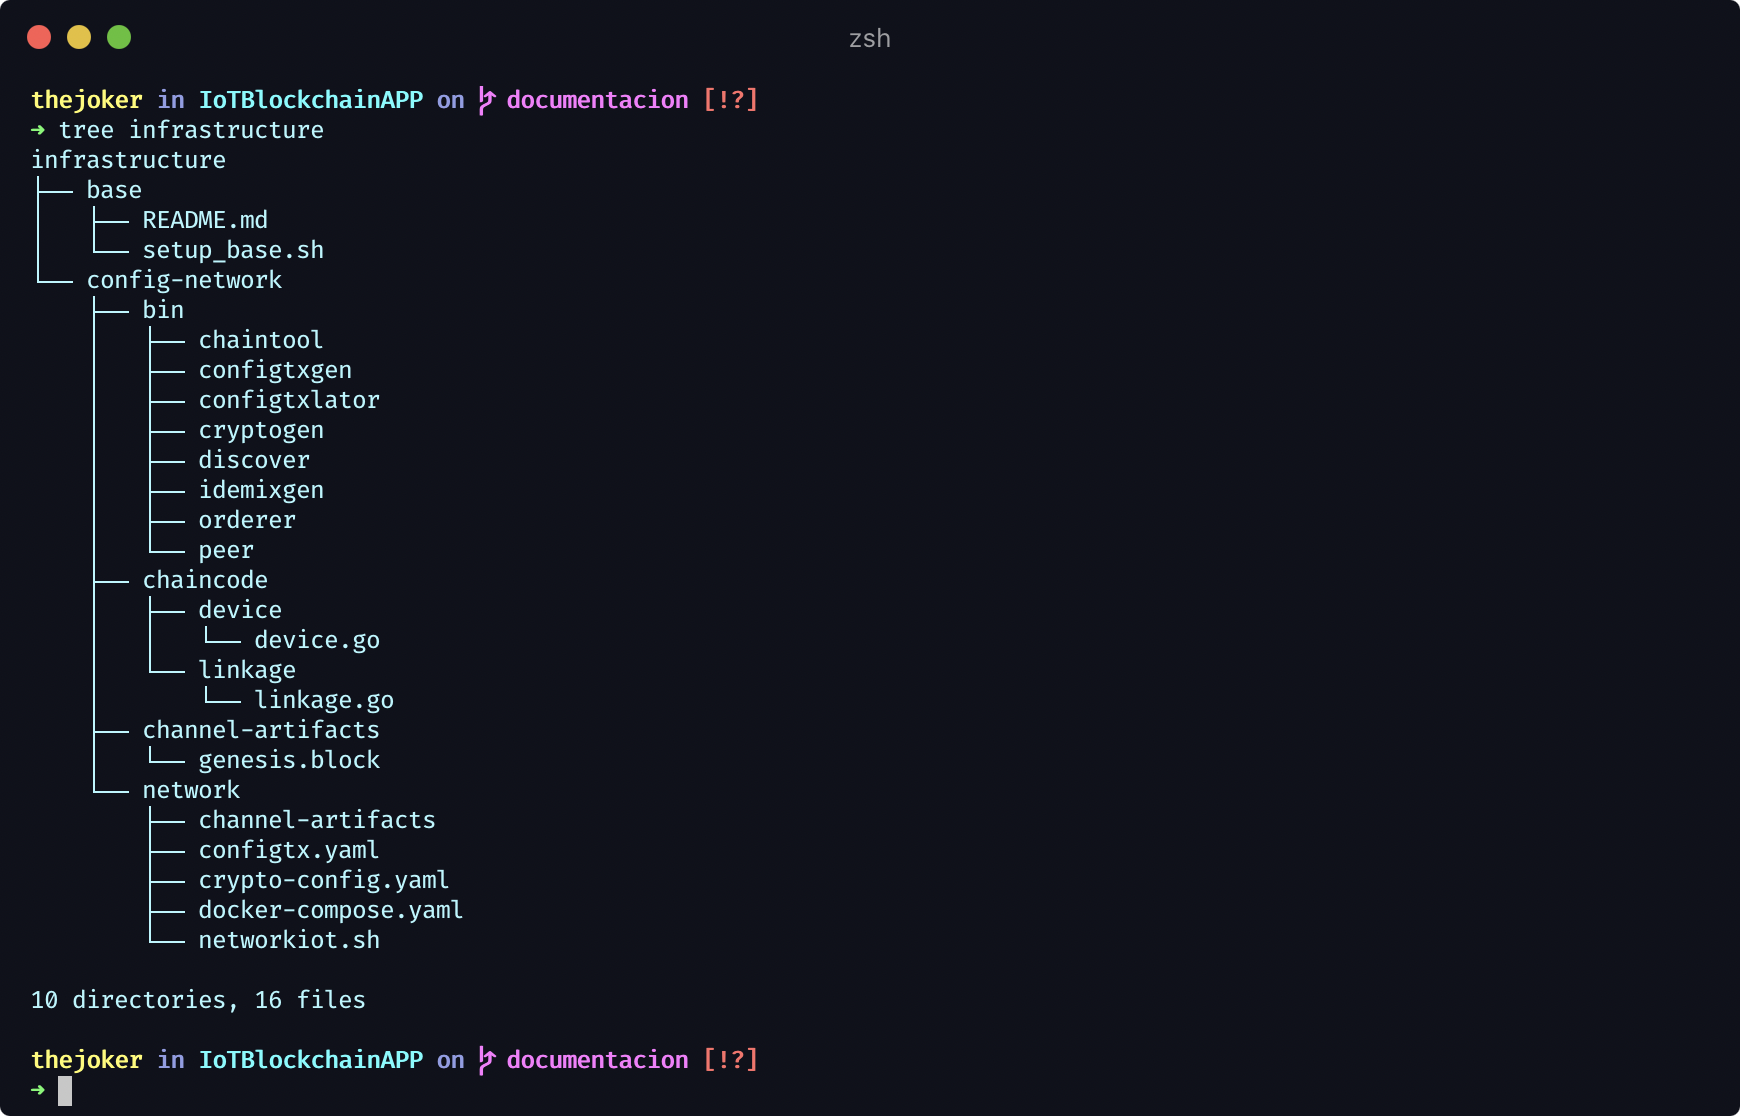
\includegraphics[width=10cm]{imagenes/desarrollo/tree_infraestructure}
  \caption{Tree de la carpeta infraestructure.}
  \label{fig:tree-infraestructure}
\end{figure}

\vspace{5mm}

\noindent La carpeta \textbf{config-network} contiene los binarios necesarios para las imagenes Docker de Hyperledger Fabric,
los chaincode creados para realizar las operaciones a los dispositivos y enlaces, y todos los ficheros necesarios para la 
configuración de la red Blockchain que son: 

\begin{figure}[h!]
  \begin{subfigure}{0.5\textwidth}
    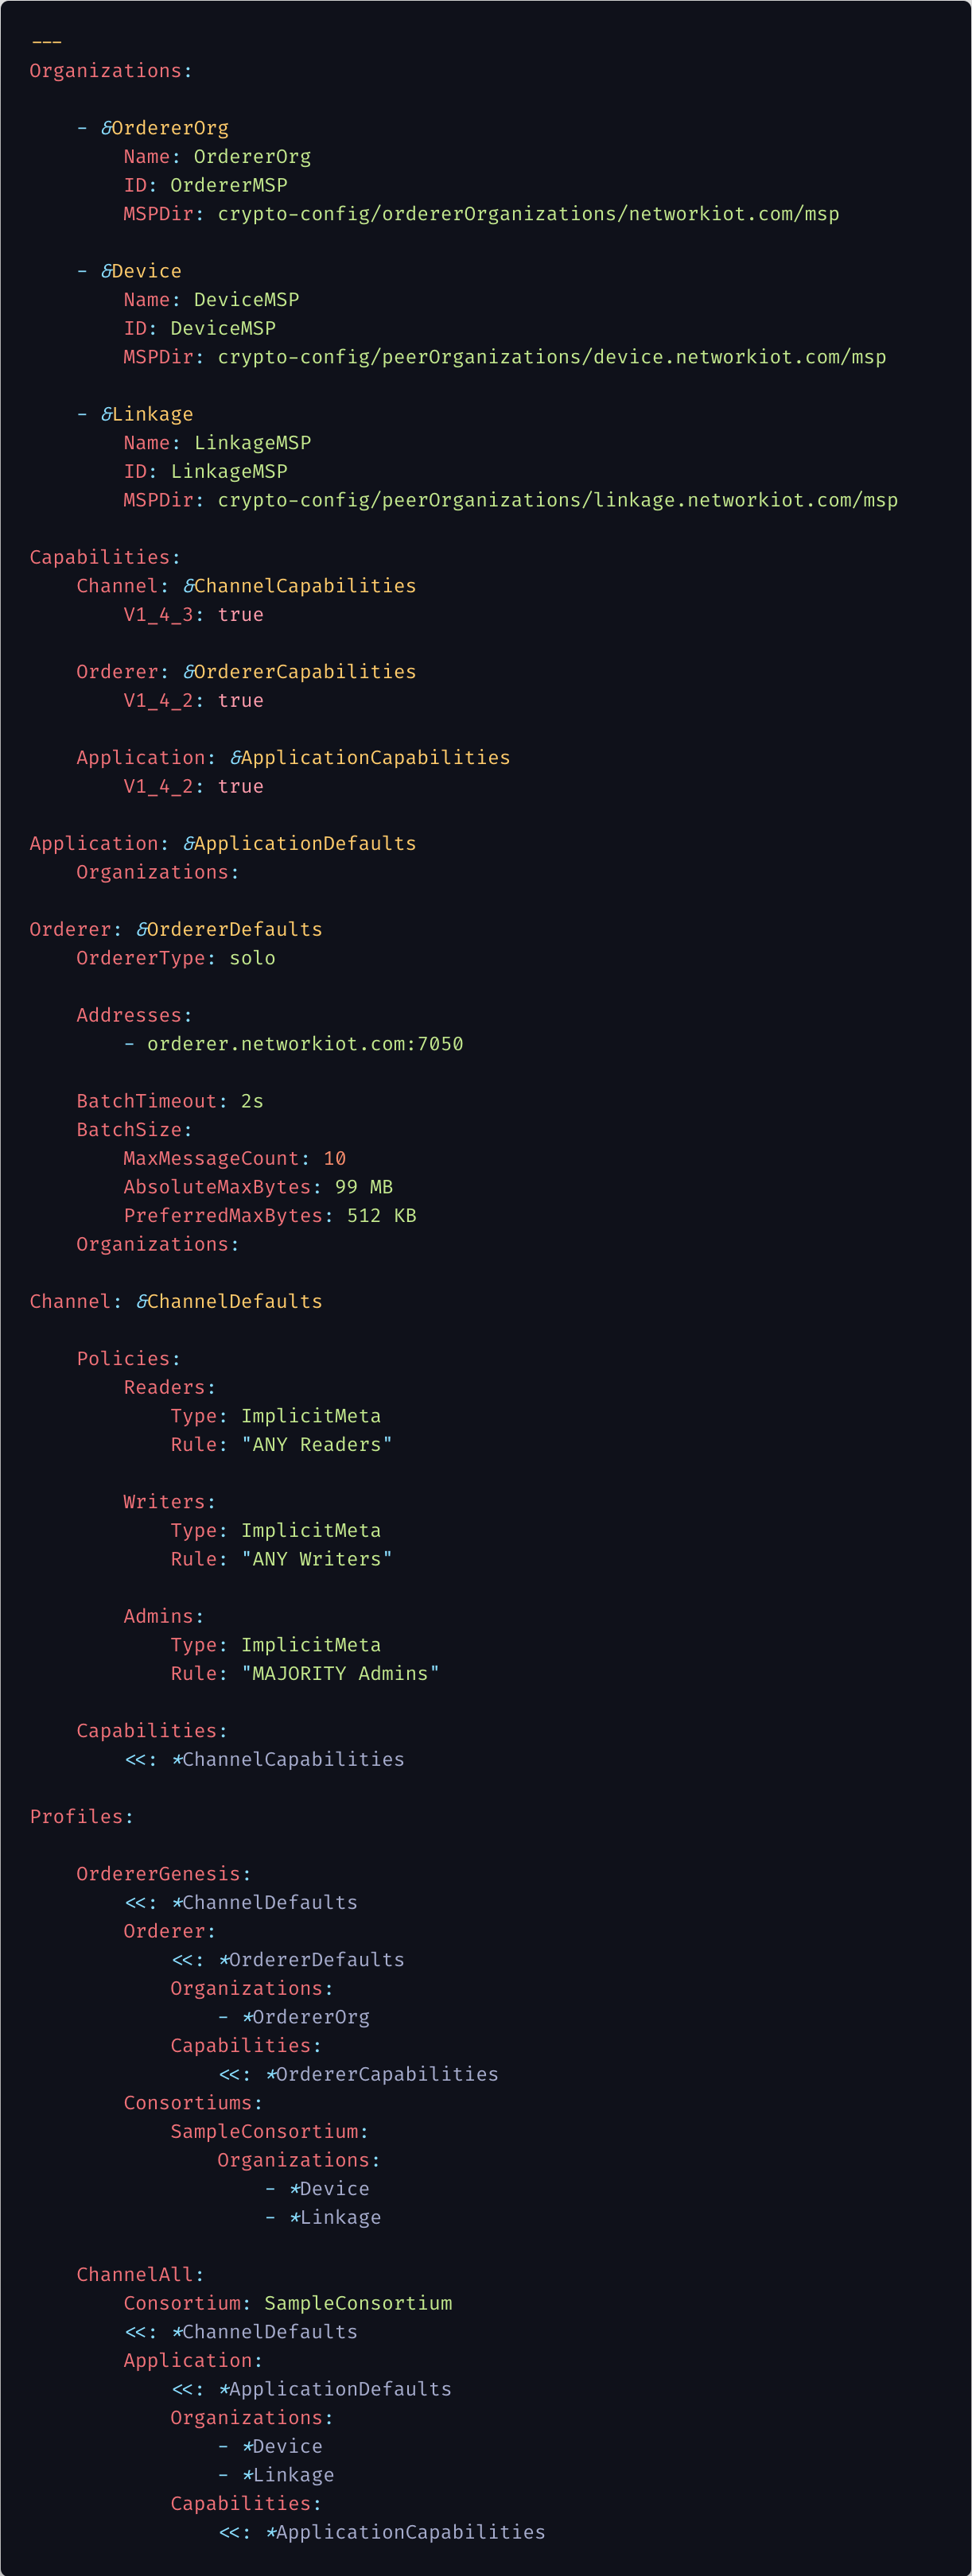
\includegraphics[width=\linewidth]{imagenes/desarrollo/configtx}
    \caption{Configtx de la red Blockchain.}
    \label{fig:configtx-blockchain}
  \end{subfigure}
  \begin{subfigure}{0.5\textwidth}
    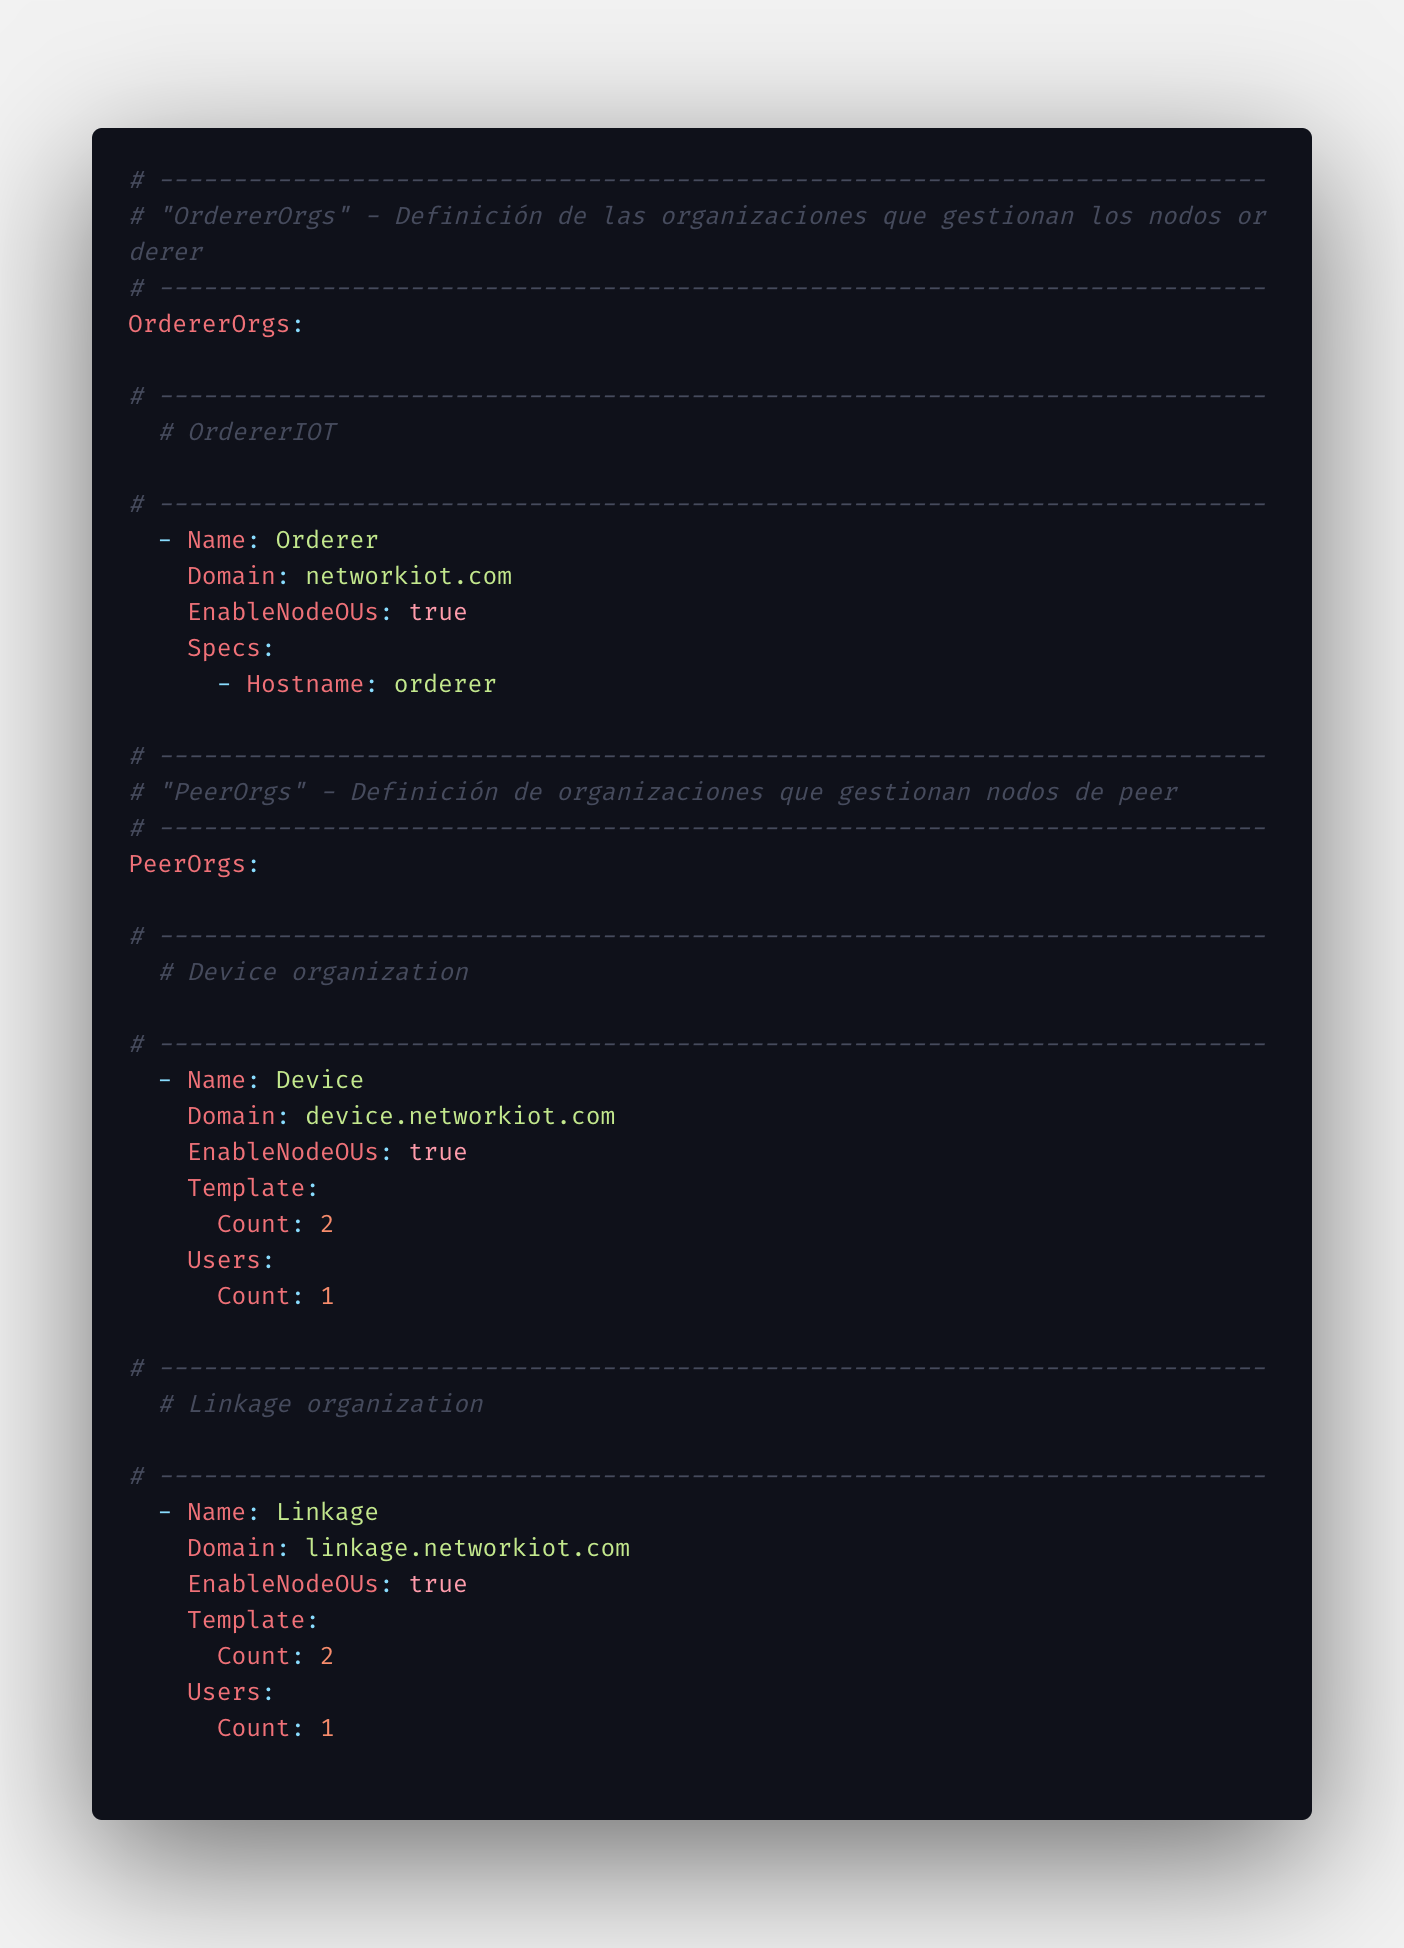
\includegraphics[width=\linewidth]{imagenes/desarrollo/crypto-config}
    \caption{Crypto-config de la red Blockchain.}
    \label{fig:crypto-config-blockchain}
  \end{subfigure}
\end{figure}

\vspace{5mm}

\noindent El fichero configtx se estructura en varias secciones, tenemos organizaciones, orderers,  aplicaciones, capacidades
y perfiles. Las secciones que podemos destacar son las organizaciones que van a formar la red Blockchain, en este caso tenemos
una organización ordered y dos organizaciones peer: \textbf{Device} y \textbf{Linkage}. Por otro lado, tenemos los perfiles donde
indicamos cuales organizaciones pueden 

\vspace{5mm}

\noindent La carpeta channel-artifacts se guardarán los archivos generados por el binario \textbf{cryptogen}, que es usado para 
la creación de los archivos de la red, pasandole como parámetro el archivo de configuración \textbf{crypto-config}. Los archivos
que se generan son:

\begin{itemize}
  \item channel.tx: archivo para la transacción de configuración del canal.
  \item genesis.block: es el primer bloque de la cadena, el bloque génesis, el cual inicia la cadena de bloques de nuestra red.
\end{itemize}

\subsubsection{Arquitectura de la red Blockchain.}

\begin{figure}[ht!]
  \centering
  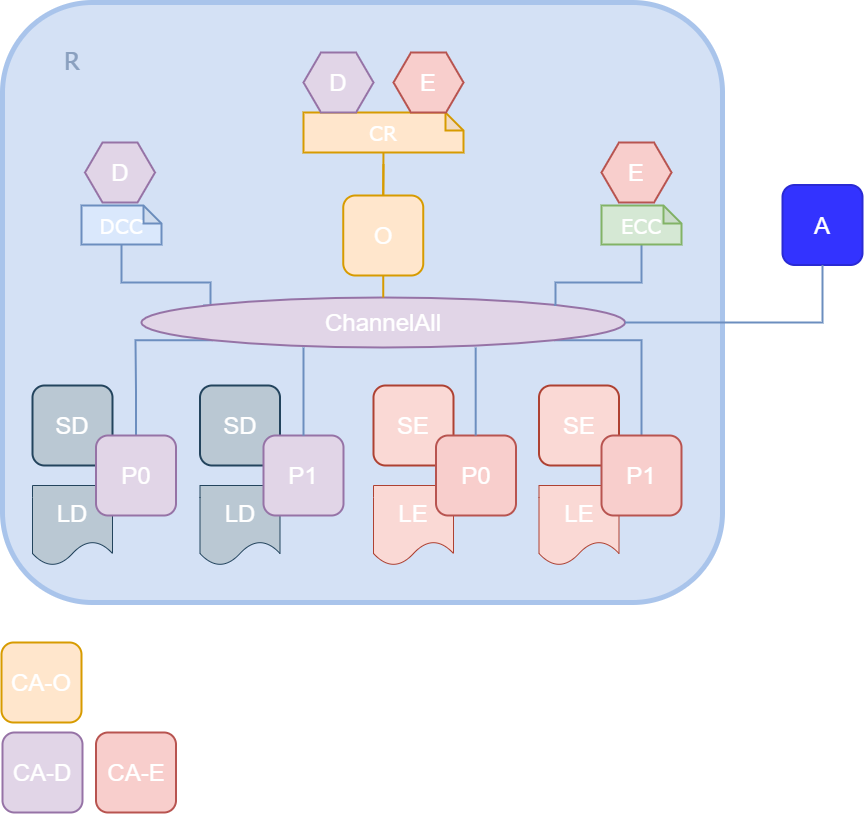
\includegraphics[width=10cm]{imagenes/desarrollo/arquitectura_networkiot}
  \caption{Arquitectura de la red Blockchain.}
  \label{fig:arquitectura-blockchain}
\end{figure}

\begin{figure}[ht!]
  \centering
  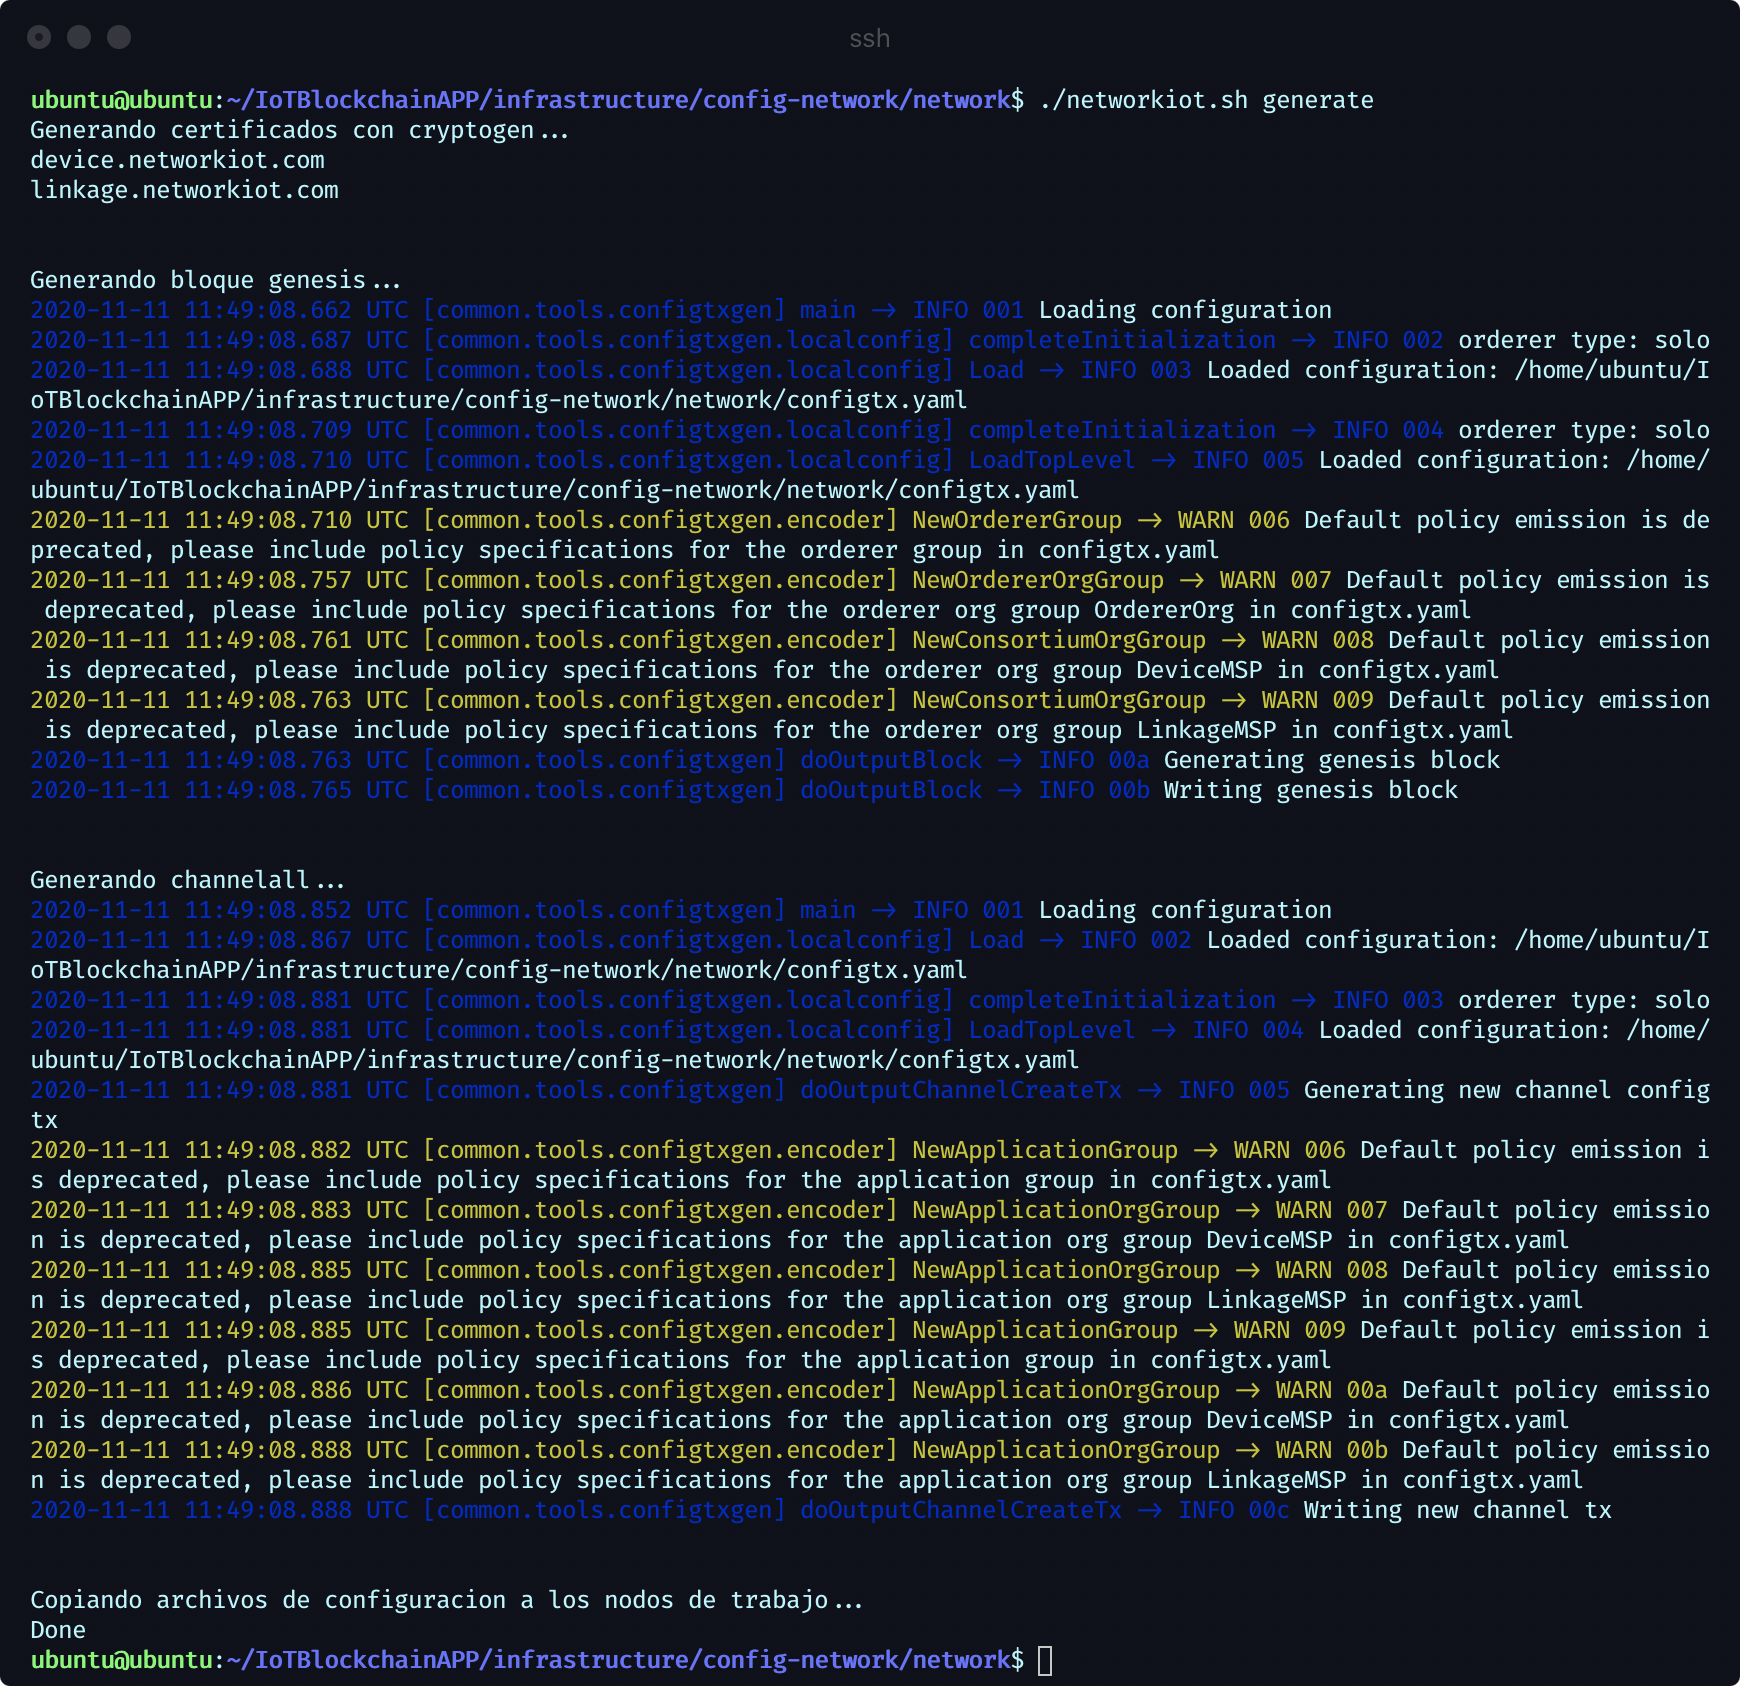
\includegraphics[width=10cm]{imagenes/desarrollo/comandos/generate}
  \caption{Opción generate del script networkiot.}
  \label{fig:generate}
\end{figure}

\begin{figure}[ht!]
  \centering
  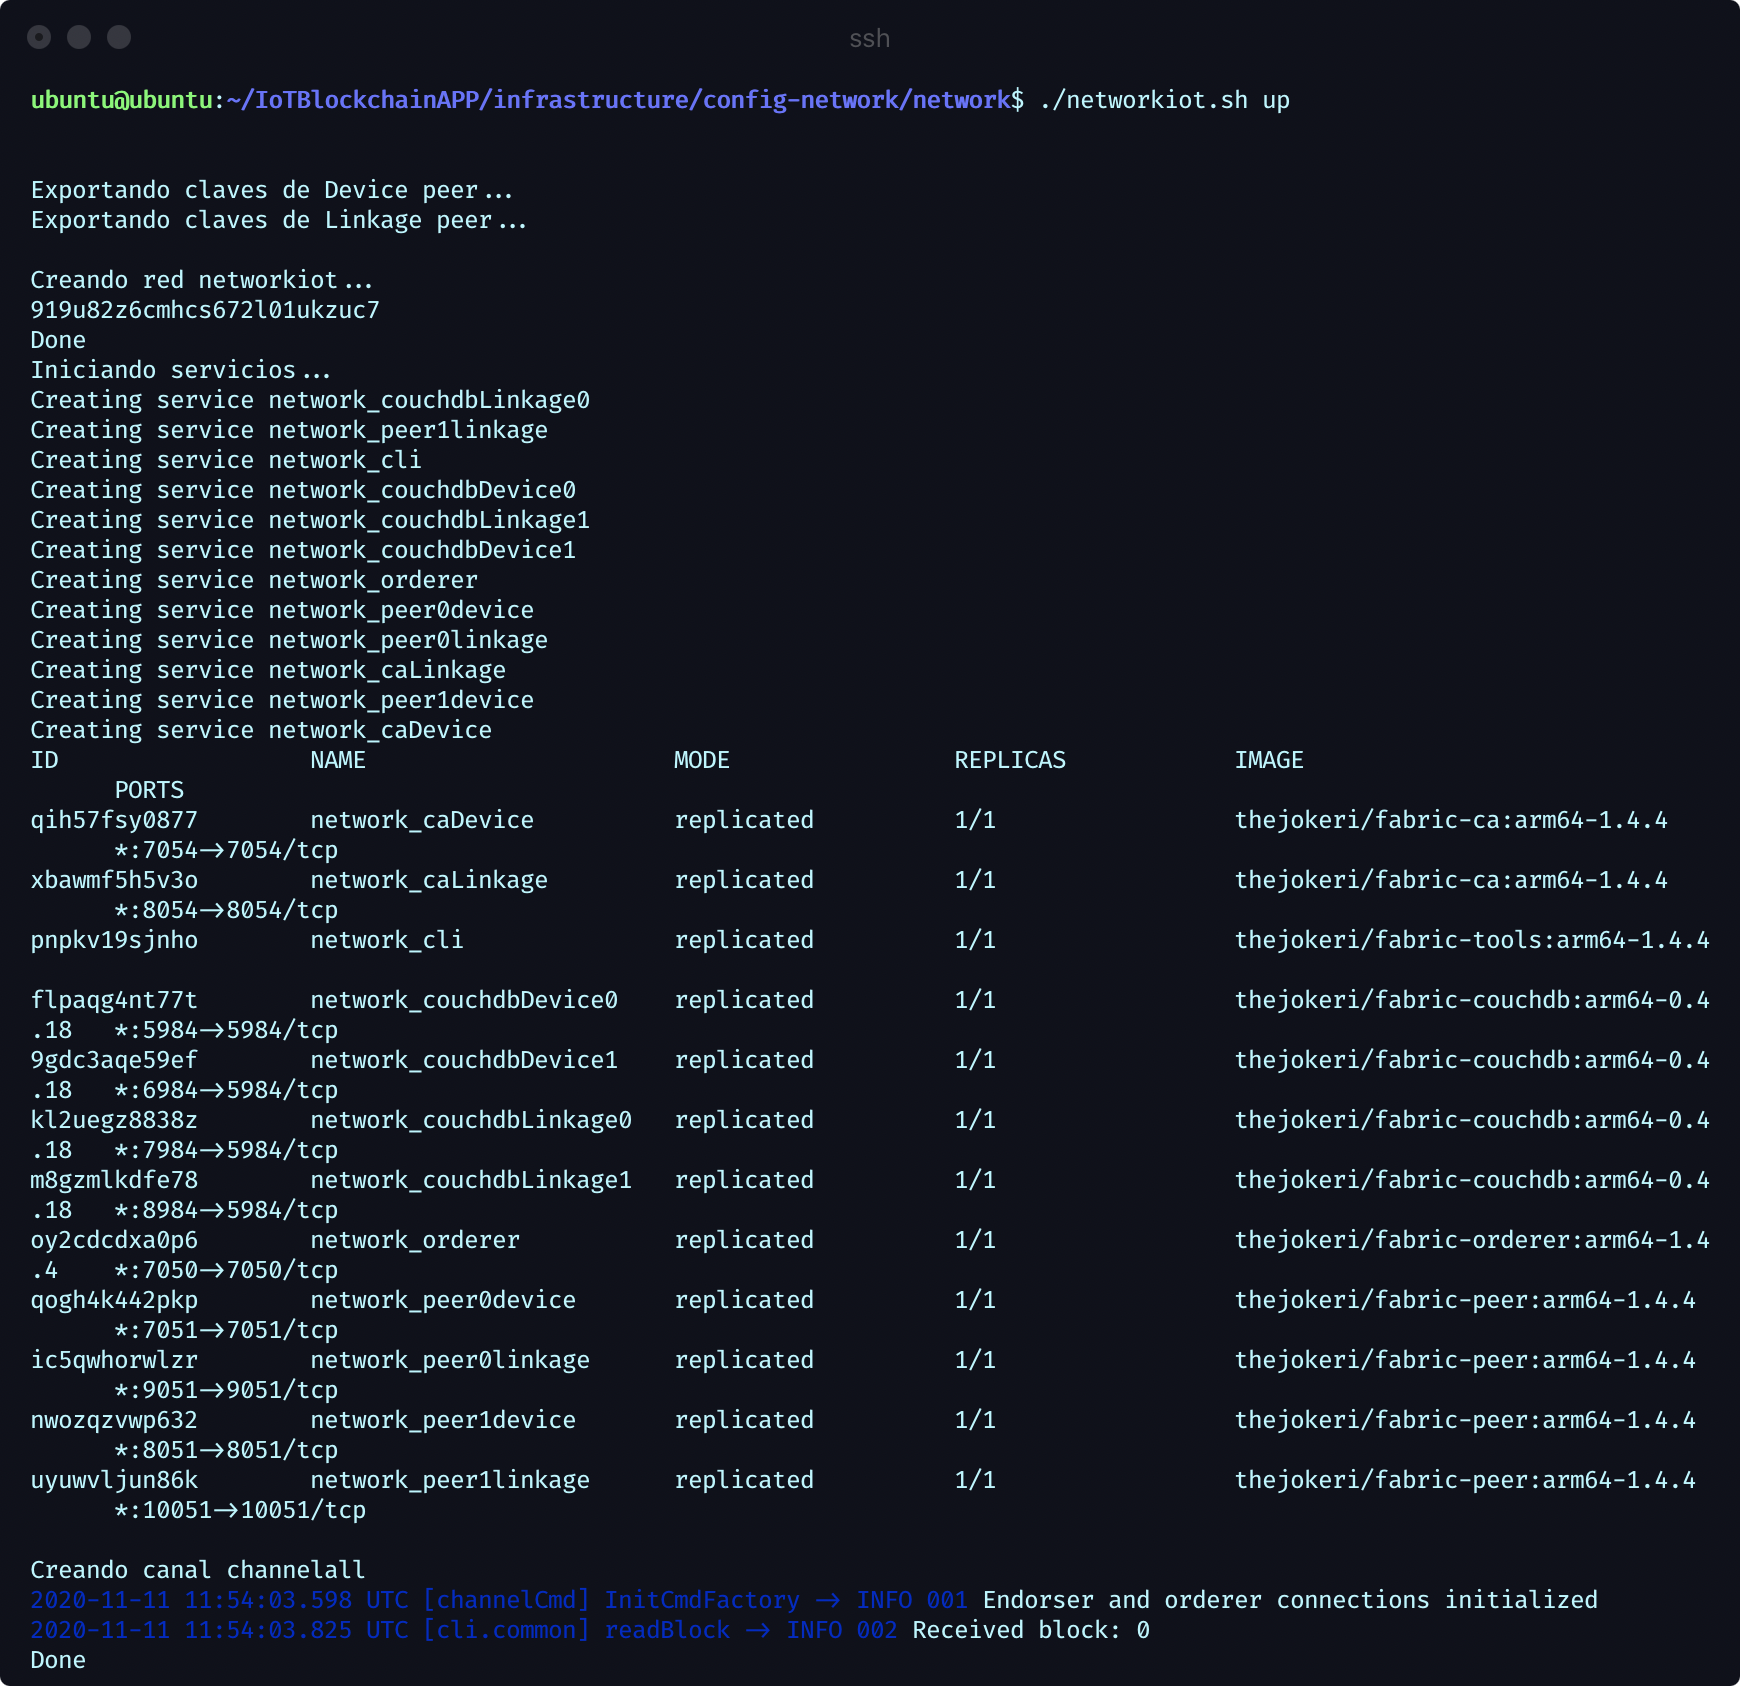
\includegraphics[width=10cm]{imagenes/desarrollo/comandos/up_1}
  \caption{Salida 1 de la opción up del script networkiot.}
  \label{fig:up-1}
\end{figure}

\begin{figure}[ht!]
  \centering
  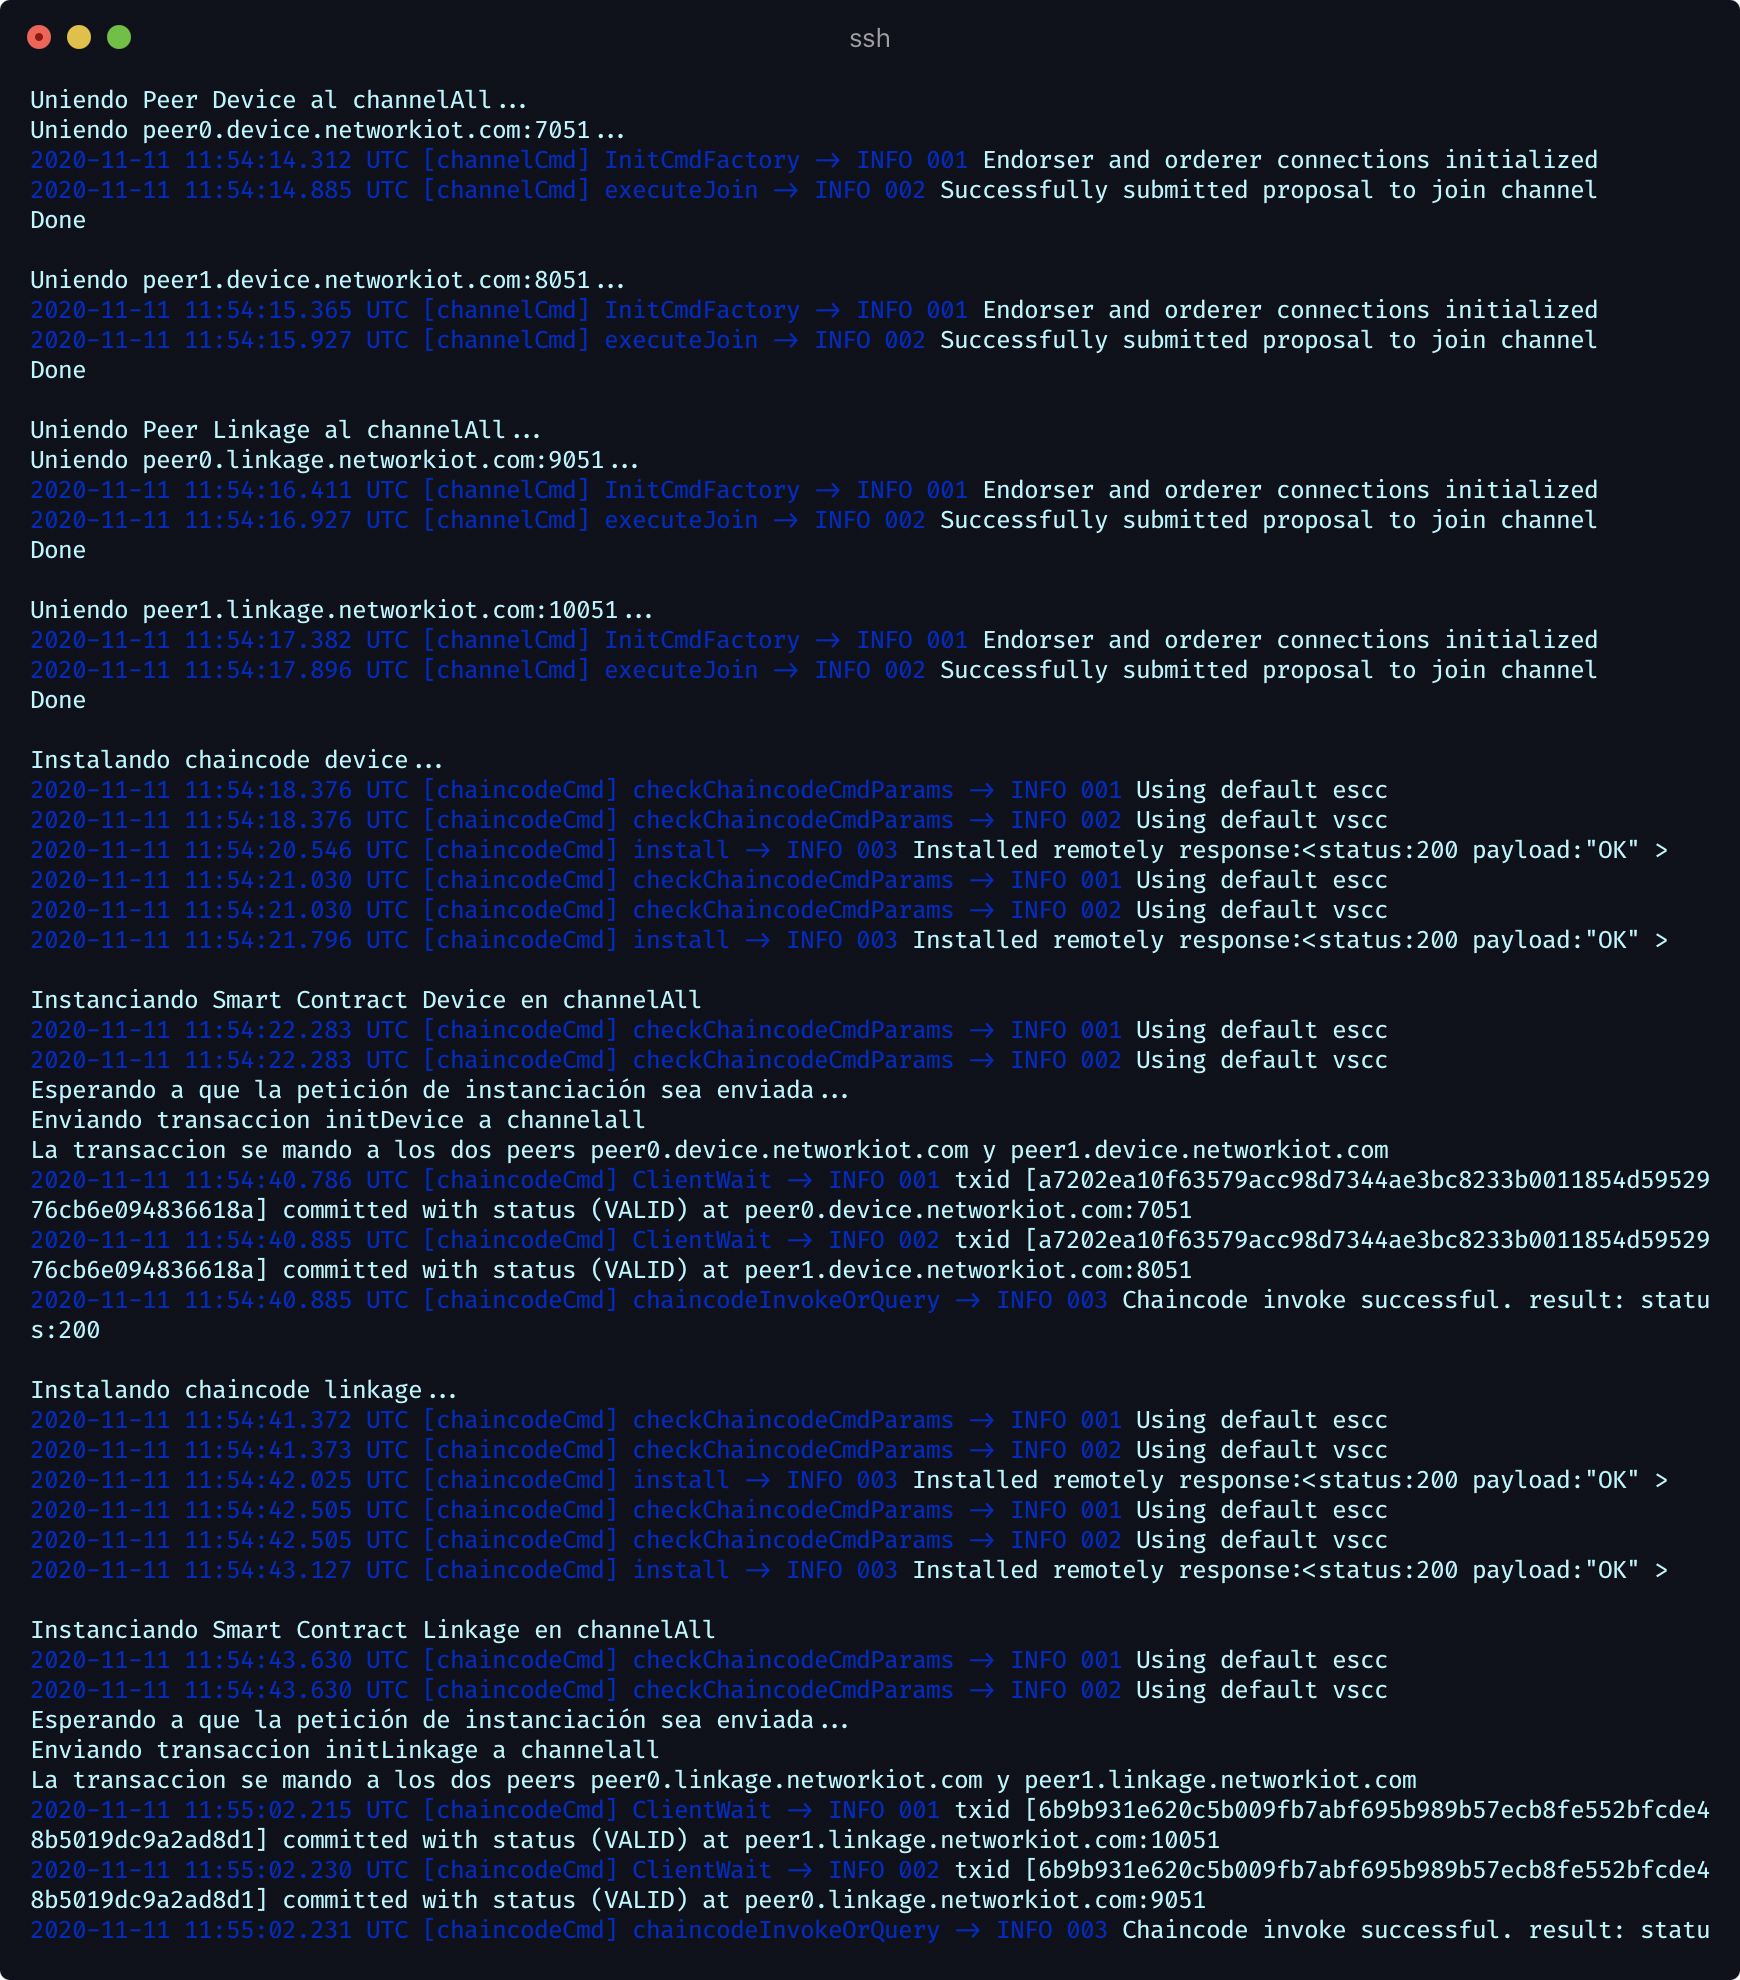
\includegraphics[width=10cm]{imagenes/desarrollo/comandos/up_2}
  \caption{Salida 2 de la opción up del script networkiot.}
  \label{fig:up-2}
\end{figure}

\begin{figure}[ht!]
  \centering
  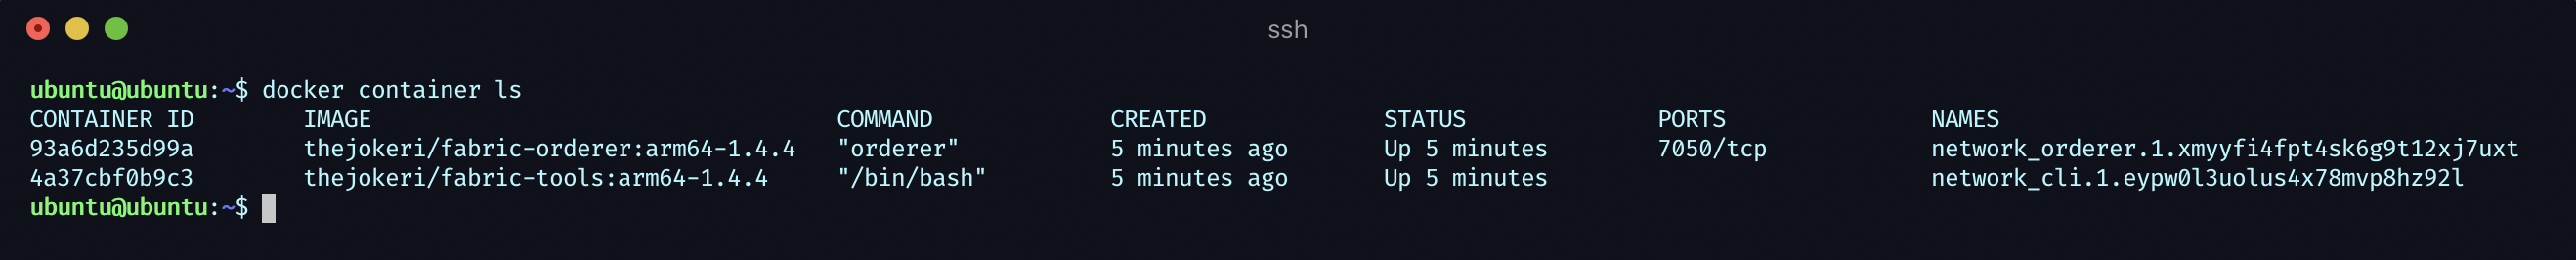
\includegraphics[width=10cm]{imagenes/desarrollo/comandos/containers_master}
  \caption{Salida de contenedores en el nodo maestro.}
  \label{fig:containers-master}
\end{figure}

\begin{figure}[ht!]
  \centering
  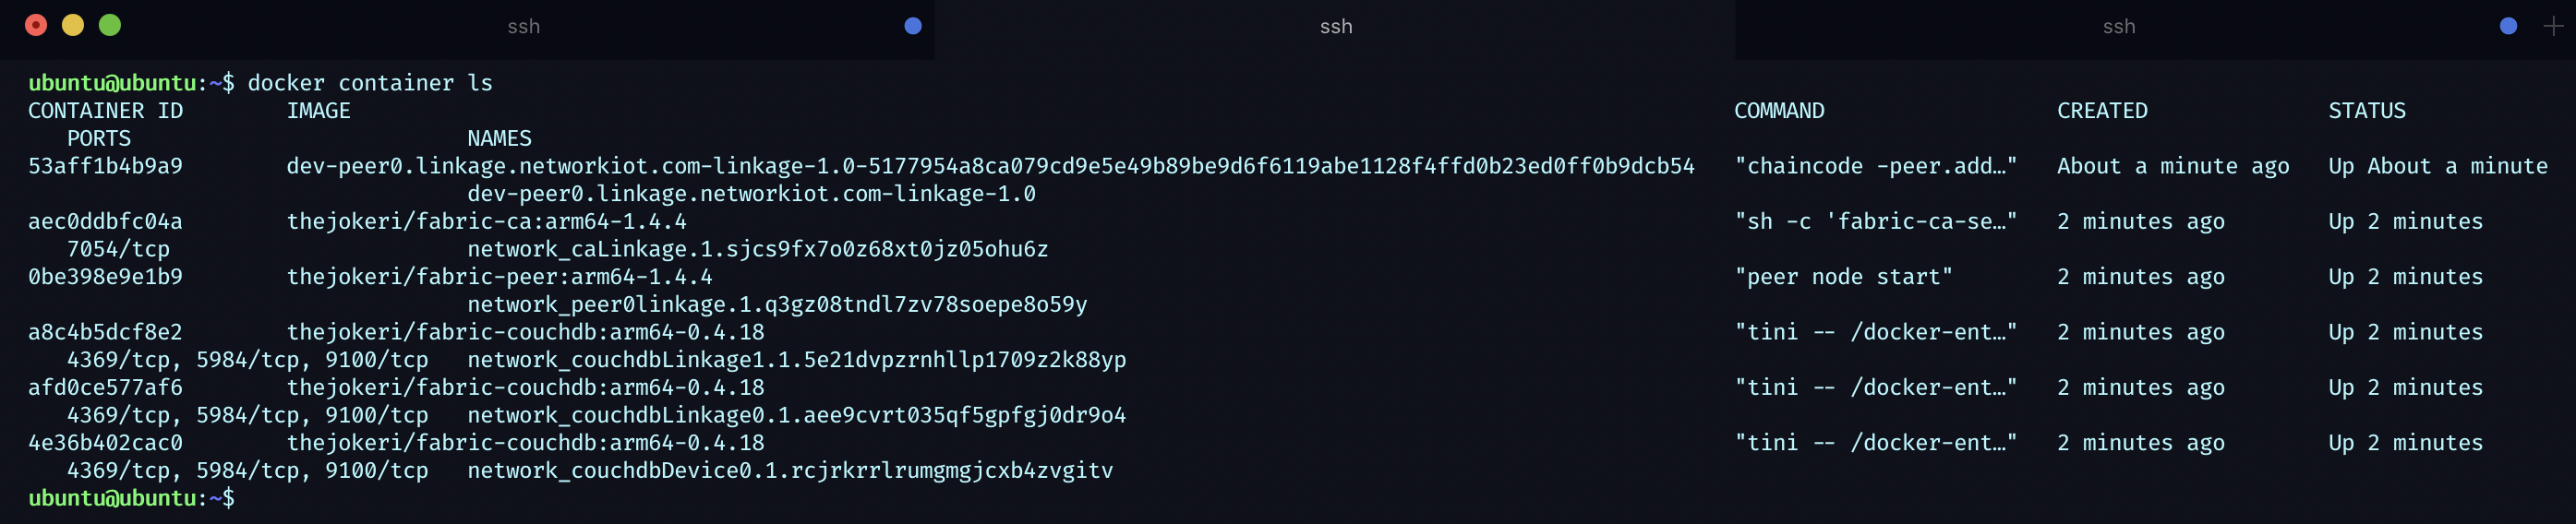
\includegraphics[width=10cm]{imagenes/desarrollo/comandos/containers_worker1}
  \caption{Salida de contenedores en el nodo worker 1.}
  \label{fig:containers-worker1}
\end{figure}

\begin{figure}[ht!]
  \centering
  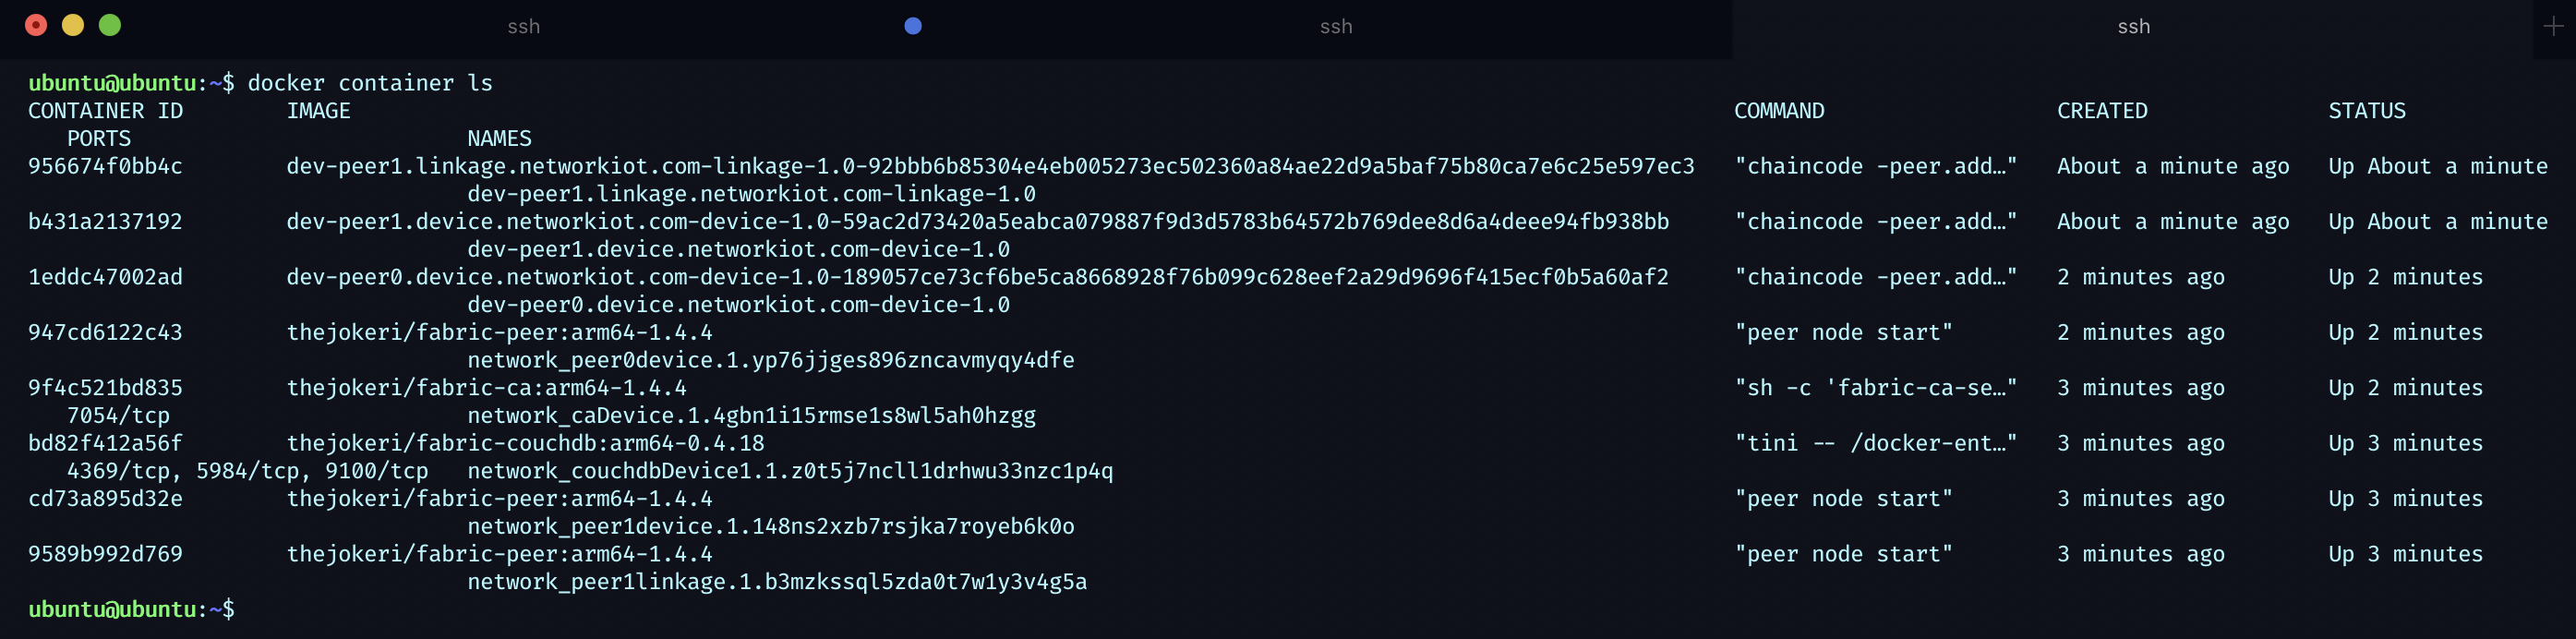
\includegraphics[width=10cm]{imagenes/desarrollo/comandos/containers_worker2}
  \caption{Salida de contenedores en el nodo worker 2.}
  \label{fig:containers-worker2}
\end{figure}

\begin{figure}[ht!]
  \centering
  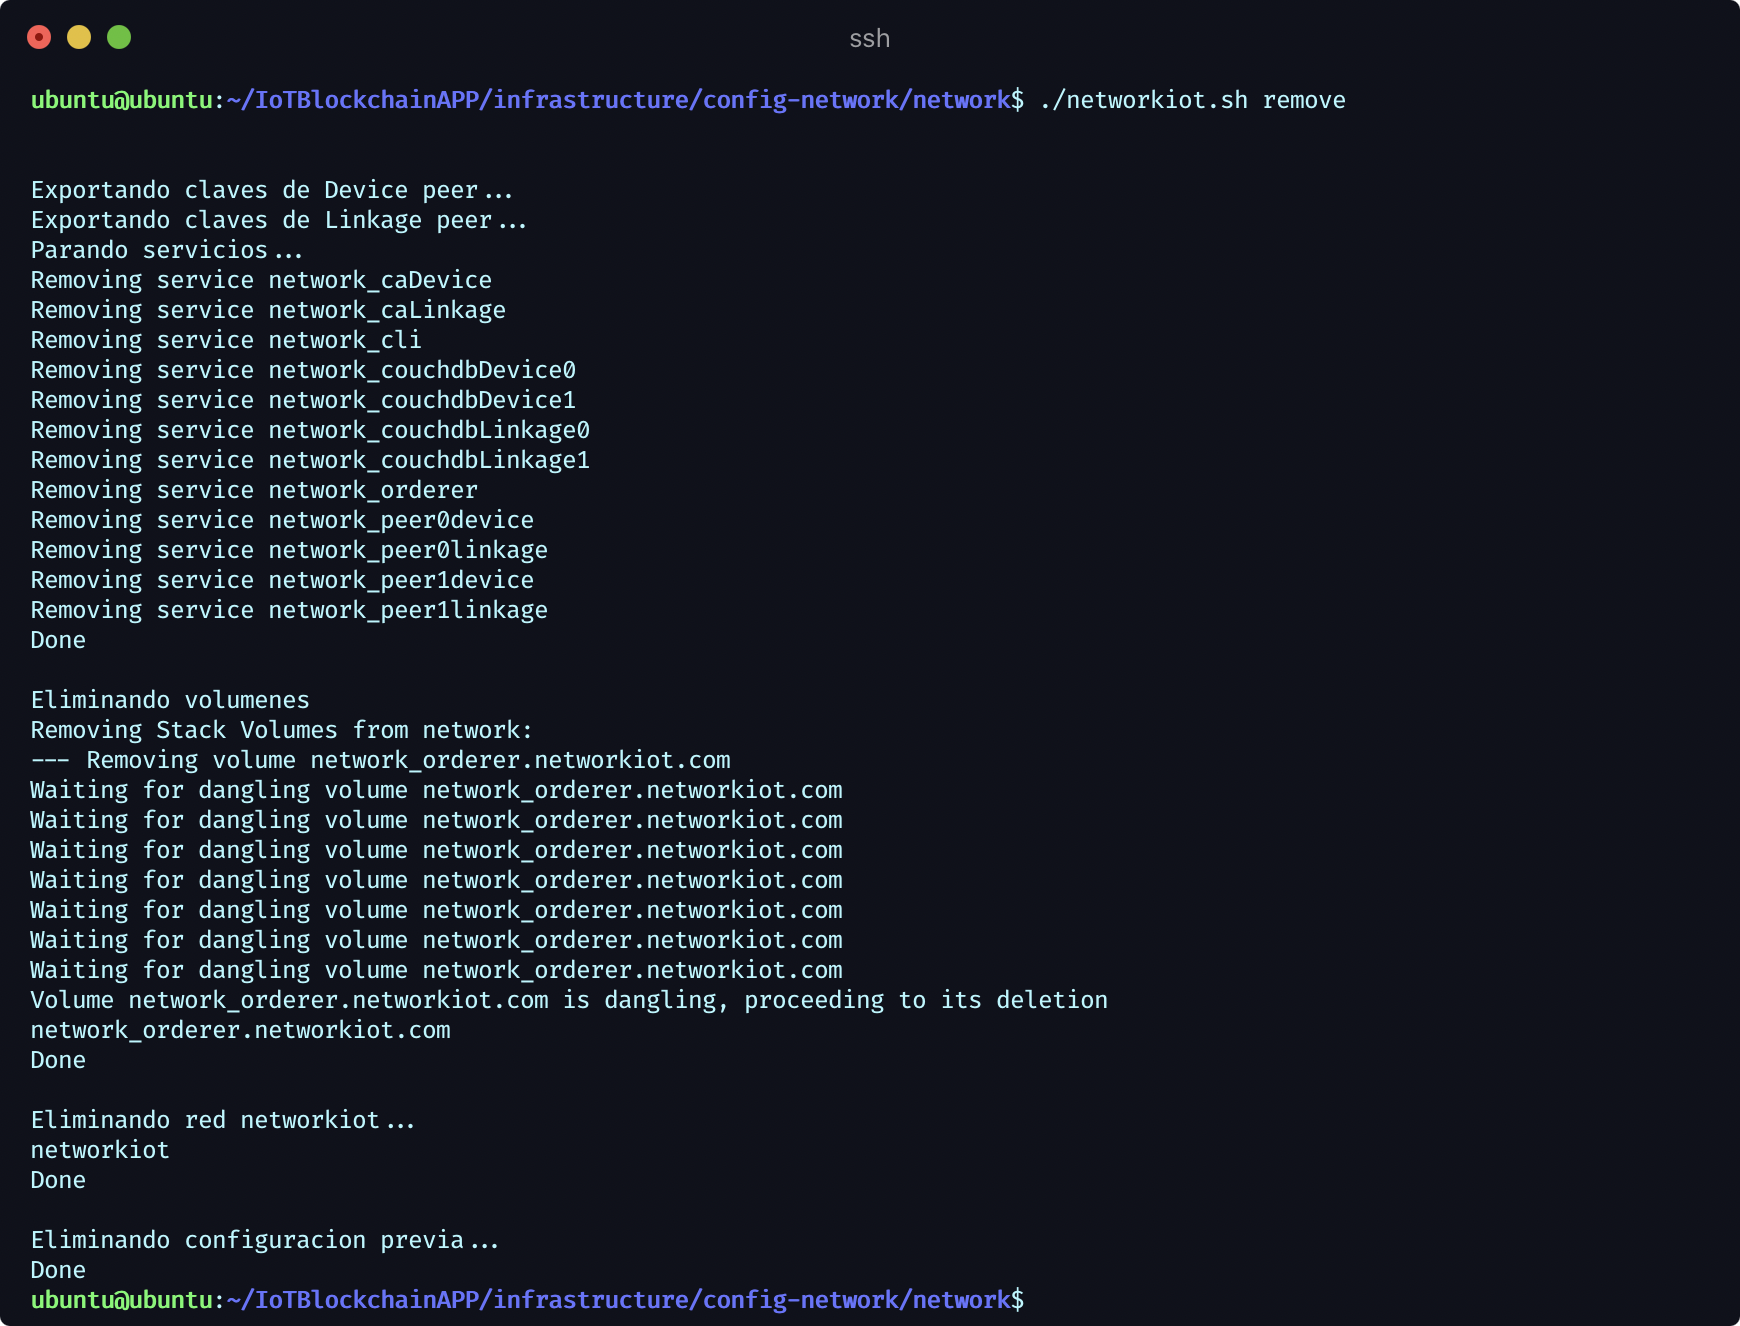
\includegraphics[width=10cm]{imagenes/desarrollo/comandos/remove}
  \caption{Opción remove del script networkiot.}
  \label{fig:remove}
\end{figure}

\subsection{Desarrollo del Back end.}

\begin{figure}[ht!]
  \centering
  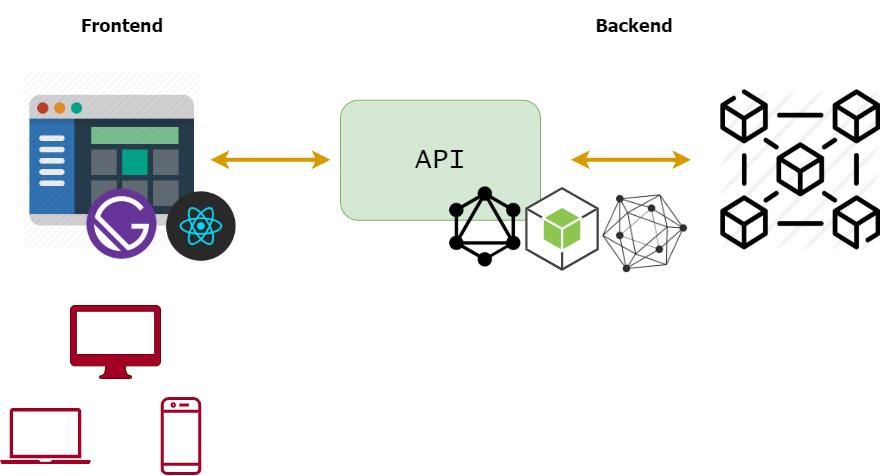
\includegraphics[width=10cm]{imagenes/desarrollo/arquitectura_aplicacion}
  \caption{Arquitectura de la aplicación.}
  \label{fig:arquitectura-aplicacion}
\end{figure}

\begin{figure}[ht!]
  \centering
  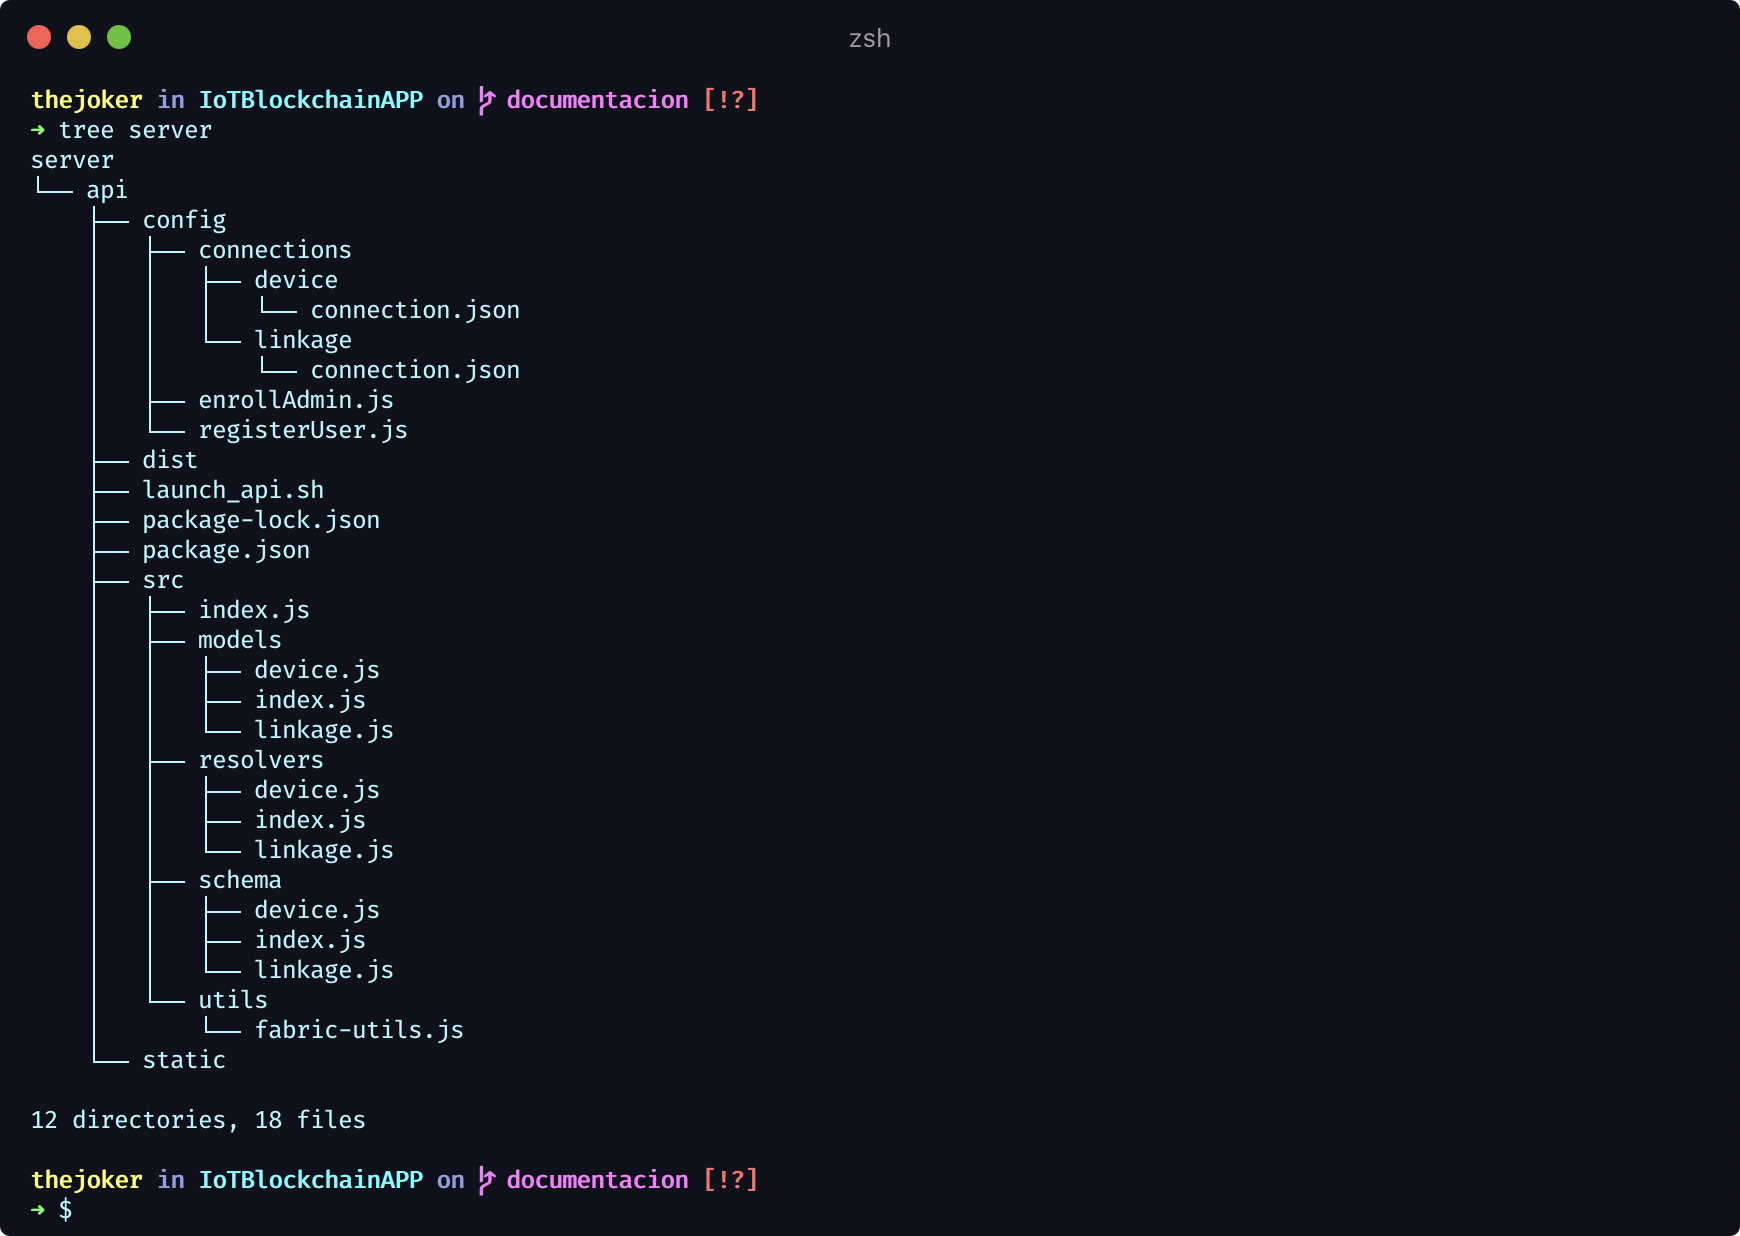
\includegraphics[width=10cm]{imagenes/desarrollo/tree_server}
  \caption{Tree de la carpeta server.}
  \label{fig:tree-server}
\end{figure}

\begin{figure}[ht!]
  \centering
  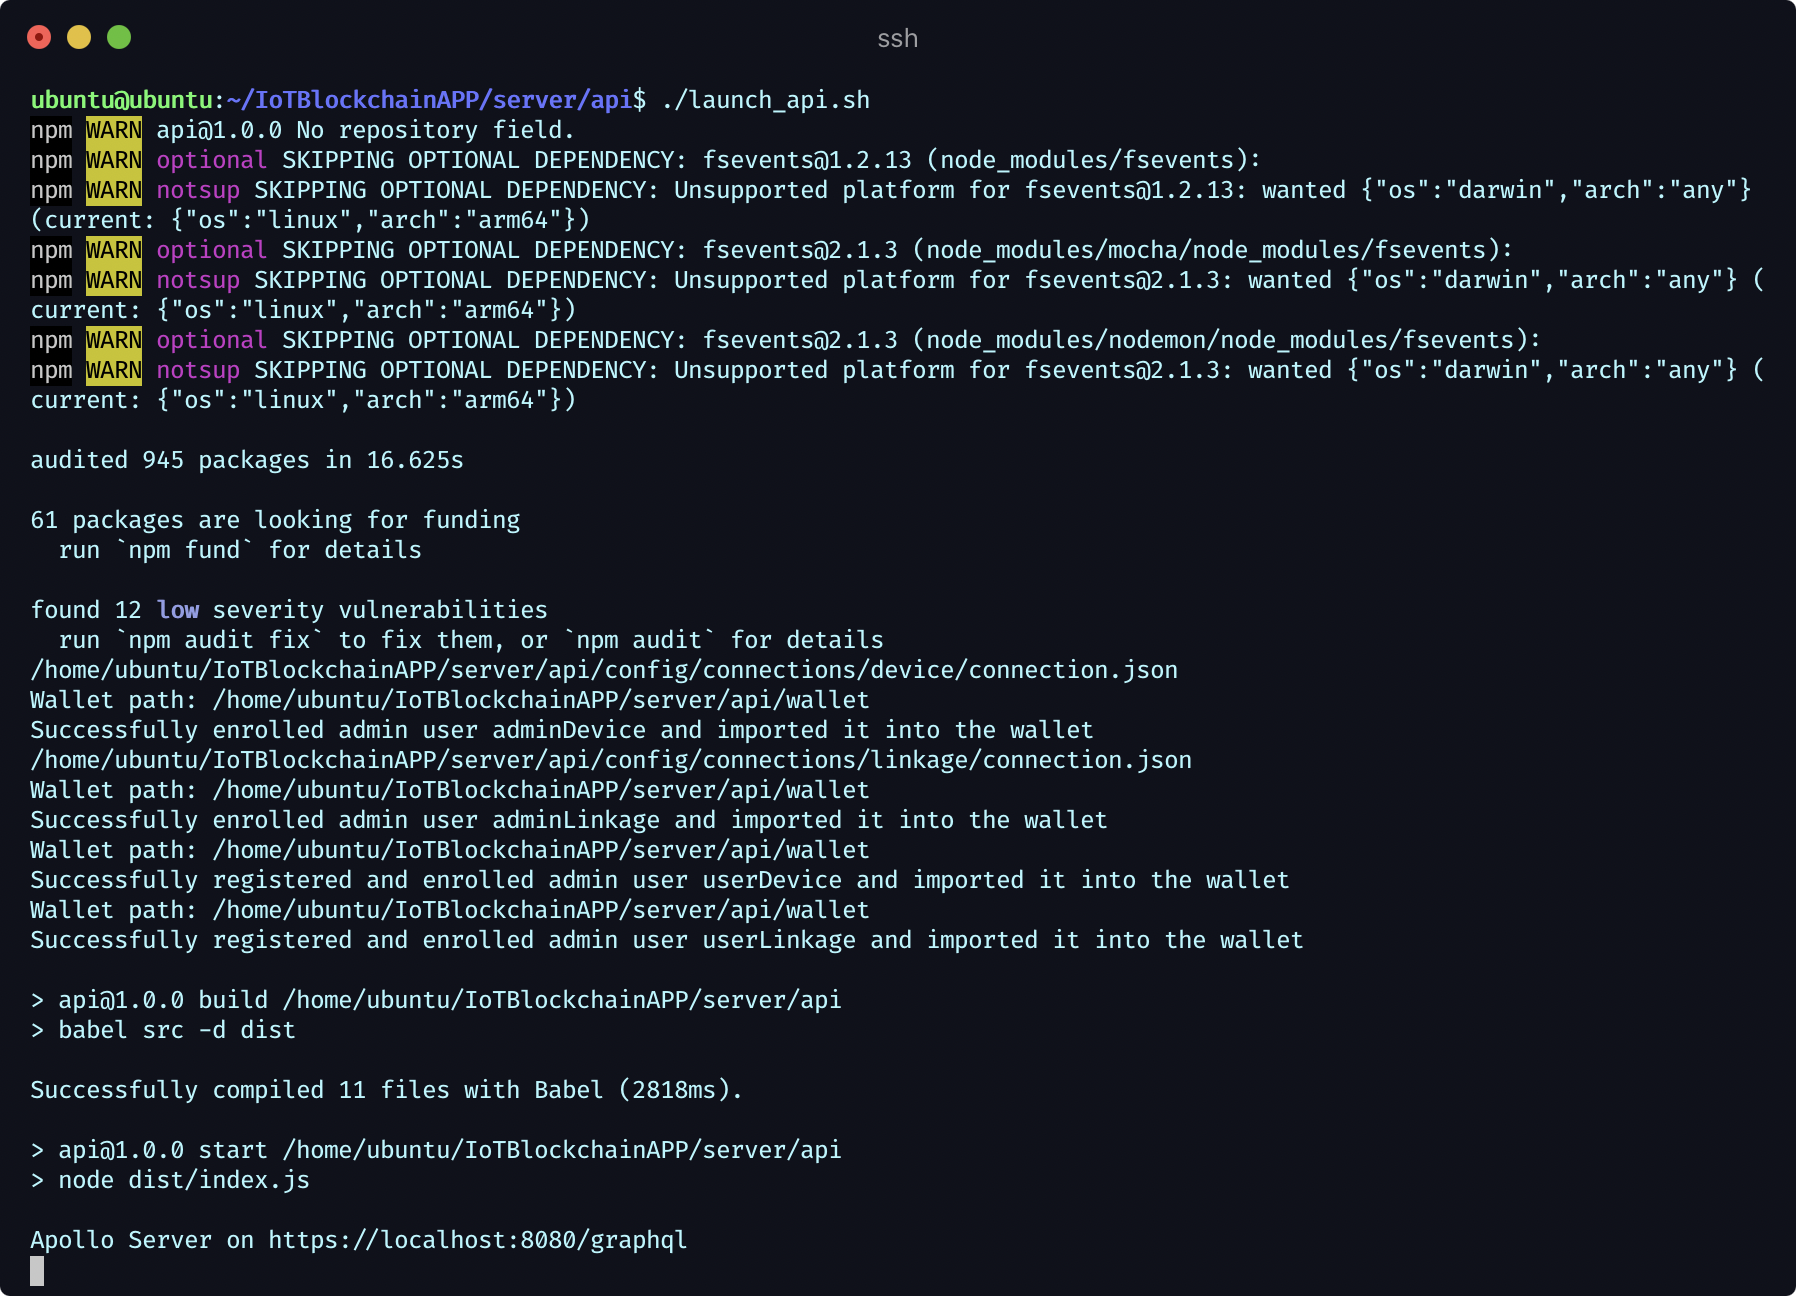
\includegraphics[width=10cm]{imagenes/desarrollo/comandos/launch_api}
  \caption{Ejecución del script launch\_api.}
  \label{fig:launch-api}
\end{figure}

\subsection{Desarrollo del Front end y despliegue.}

\begin{figure}[ht!]
  \centering
  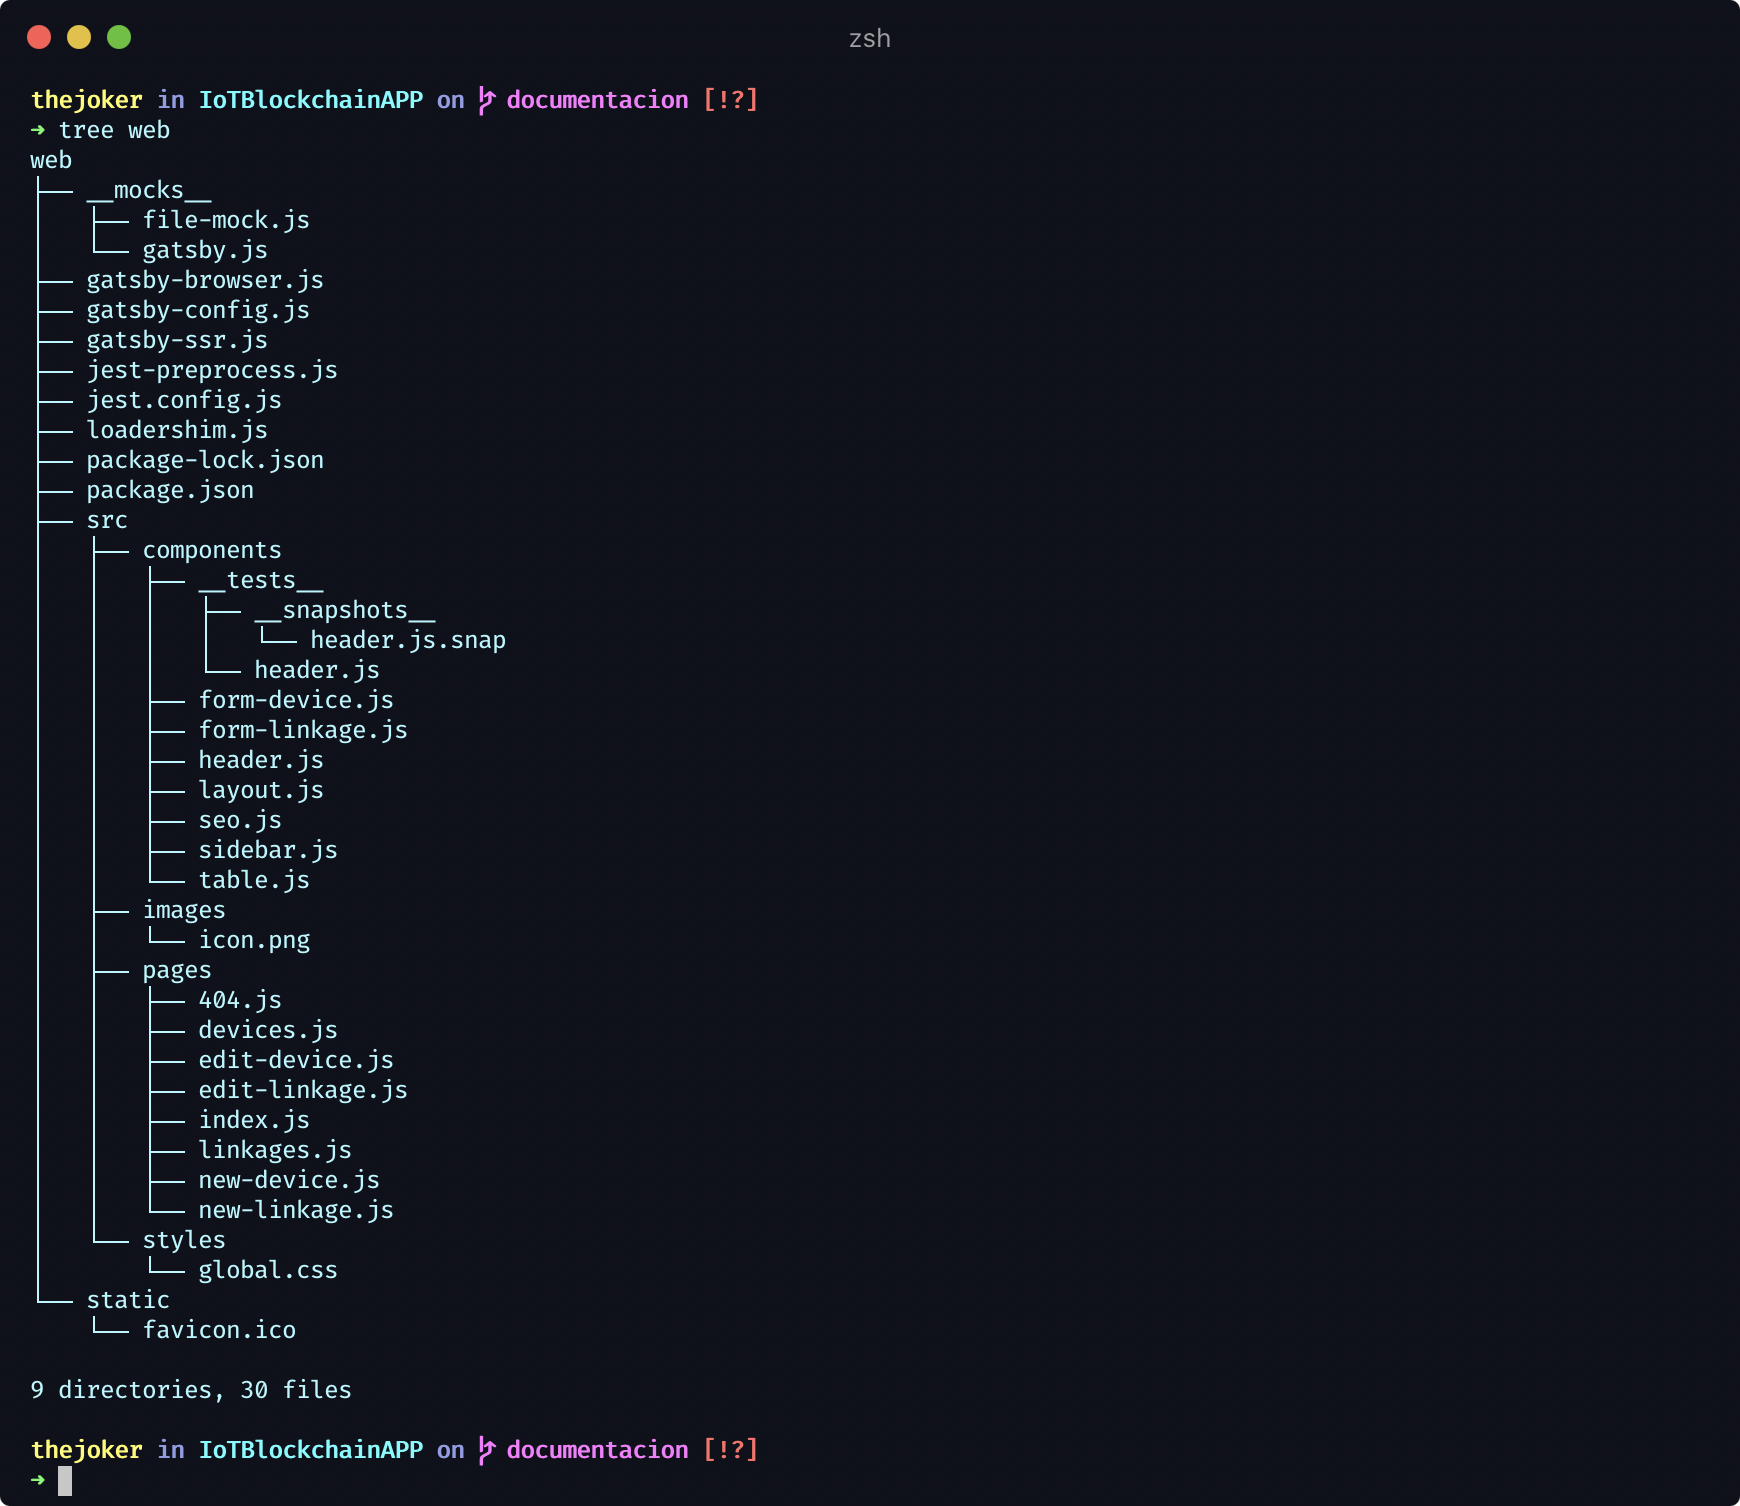
\includegraphics[width=10cm]{imagenes/desarrollo/tree_web}
  \caption{Tree de la carpeta web.}
  \label{fig:tree-web}
\end{figure}

\subsection{Conclusión.}

\newpage